%% Classe du document
\documentclass{article}
%\documentclass[]{report}

\usepackage{preambule_all181211}

\graphicspath{{figures/}{../figures/}}

\begin{document}
\maketitle

%%%%%% INTRO
	%%!TEX root = ../ArticleCalib_main.tex

%%%%%%% INTRODUCTION article calib
\section{Introduction}

In the recent years, increasingly sensitives detectors are used to detect localised sources, like small objects or single molecules, but those low noise point detectors are unsuitable for extended sources or diluted emitters. 
Infra-noise light fluxes produced by an extended surface needs larges light detectors ; however increasing the surface of a detector increases its noise, and its noise's variance.

Among all detectors, there are many advantages of EMCCDs, such as sub-electron read-out noise and low dark current, for low light applications. Nowadays their low areal noise and high detection capacities permit to reach single photon detection ; however, detecting a few photon per hour stays a challenge, more so when emitted by a large surface. To achieve a sufficient signal over noise ratio (SNR) for significative detection, one must carefully consider and explore the operating mode of the camera, to reach a detection's optimum for a given light flux.

In our work, we address the detection a light flux intensity (1 photon/sec/cm$^2$) given by a large area, as compared to the sensor's surface, which is lower than our detector equivalent areal noise. % combiner les deux

Concerning light flux detection, 3 situations have to be considered :
\begin{itemize}
\item constant uniform flux,
\item variable uniform flux :  statistic filtering,
\item non uniform flux : detection of an object's presence.
\end{itemize}

Here, we propose a statistical method, combined with an EMCCD detector, for an optimised detection of constant, uniform, and low light fluxes emitted by dim extended objects.
We present the camera we choose and its use's mode,  describe the statistical model of the detector, and show the experimental pixel by pixel characterisation and behaviour of the detector. 
Then we build a model to simulate the detector's response to a low, constant, uniform flux, and to extract the SNR as well as two characteristics exposure times, in order to use the detector optimally.







	
%%%%%% CAMERA PRESENTATION
	%%!TEX root = ../ArticleCalib_main.tex

%%%%%%% CAMERA PRESENTATION article calib
\section{Camera Presentation}










	
%%%%%% DETECTOR STATISTICAL MODEL
	%%!TEX root = ../ArticleCalib_main.tex

%%%%%%% MODEL STAT article calib
\section{Statistical model}

A SNR model was built to evaluate the sensitivity to detect a uniform light flux impinging on the detector. To this end, the measured observable is simply the total number of counts on the detector N1, i.e. the number of pixels that light up. 
It amounts to using the whole detector surface as a single big pixel, and provides us with an outstanding sensitivity.\par
 
As the detector is operated in the photon-counting (PC) mode, the output of each pixel, 0 and 1, is a simple Bernoulli random variable, $X_{pixel}$, if considering independent repetitions over time.
Each pixel having its own CIC and I$_{dark}$, the probability to light up can be broken into the probability to deliver a CIC count $p(X_{}=1)$ or a dark count $p(X_{dark}=1)$.  A simple reasoning leads to : 

\medskip
\centerline{$p(X_{pixel}=1) = 1- p(X_{pixel}=0)= 1-  p(X_{CIC}=0)*p(X_{dark}=0)$}
\medskip
 
$X_{CIC}$ is considered as a simple stationery Bernoulli variable, and $X_{dark}$ as a Bernoulli variable depending on the exposure time.
More precisely, the dark count during a given exposure time is assumed to be poissonian, from which $X_{dark}$, which is binary, is truncated. As a consequence :  

\medskip
\centerline{$p(X_{pixel}=0) = (1-p_{CIC}) * e^{- \lambda \tau}$}
\medskip
 
where $\lambda$ is the frequency of counts as a result of the additive effect of the dark current and the light flux  $\phi = \phi_{I_{dark}} + \phi_{signal} $.
Since this is a Bernoulli variable, the variance is :

\medskip
\centerline{ $\sigma^2_{Id+CIC} = P_{Id+CIC} * (1-P_{Id+CIC})$ }
\medskip
 
and the SNR reads :

\medskip
\centerline{$SNR = \frac{\Delta_{(signal+noise)-noise}}{\sqrt{\sigma^2_{signal+noise}+\sigma^2_{noise}}}$}
\bigskip

The SNR for the sum of all pixels N1 is represented as a of function of the time of exposure for different values of $\epsilon = \phi_{signal}/\phi_{I_{d}}$, ratio of the signal flux over the equivalent dark flux.

	
%%%%%% CARACTERISATION OF SINGLE PIX RESPONSE
	%%!TEX root = ../ArticleCalib_main.tex

%%%%%%% CARACTERISATION OF SINGLE PIX RESPONSE article calib
\section{Single pixel response's characterisation \label{sec:SinglePixCaract}}

When considering the image obtained from a very dim object, the problem is to distinguish if a pixel or an area of pixels is significantly higher (or not) than the neighbours. In other words, is a pattern of pixels (zeros and ones) consistent with the random effect of a perfectly uniform optical field, or is it produced by a contrasted object ? 
To address an heterogeneous light flux detection, it is essential to know the background and the fluctuations of each pixel one by one. \par

We studied the camera pixels with the following steps. 
First, studying the global response of the detector (ones' frequency per frame for a given exposure time), gives a preliminary approach of the real CIC and $I_{d}$ of our camera (\ref{fig:PixByPix:A}).
Second, we determined for each pixel the CIC and the $I_{d}$ by a linear regression for exposure times that stay away from saturation ( \ref{fig:PixByPix:B}). For the linear regression, we weighted the estimated variance of each data point, and were satisfied with the goodness of fit ($\chi^2$, data not shown.) 
Then we observed the distribution of the  CIC and the $I_{d}$ parameters across all pixels (\ref{fig:PixByPix:B}), leading to a histogram (\ref{fig:PixByPix:F}, \ref{fig:PixByPix:G}) and cumulative distribution (\ref{fig:PixByPix:D}, \ref{fig:PixByPix:E})  and an image (data not shown) for each parameter. Abnormal pixels were localised on the camera chip, and subsequently discarded when needed.\par

The heterogeneity of the sensor shows outliers of lower $I_{d}$ (2\textperthousand, 513$^e$ line) and higher $I_{d}$, (1\textperthousand, randomly spread on the sensor), as well as pixels of higher CIC, patterned in pixels columns, with outliers among them ($\tilde{F}_{CIC} > 5.10^{-3}$ : 1\textperthousand, 513$^e$ line.) However, 99\% of the detector is homogeneous, with a noise variation coefficient $c_v$ such as $c_v_{CIC}$ = 0.32 and  $c_v_{Id}$ = 0.34. \par
\medskip

%%!TEX root = ../ArticleCalib_main.tex
%!TEX root = ../sections/articleCalib_section4_SinglePixResponse

%%%%%%% FIGURE 1  : SINGLE PIX RESPONSE / HISTO CDF

\newgeometry{top=10mm}

\begin{figure}[]
\begin{center}
\captionsetup[subfigure]{position=top, labelfont=bf, textfont=normalfont, singlelinecheck=off, justification=raggedright }

\subfloat[]{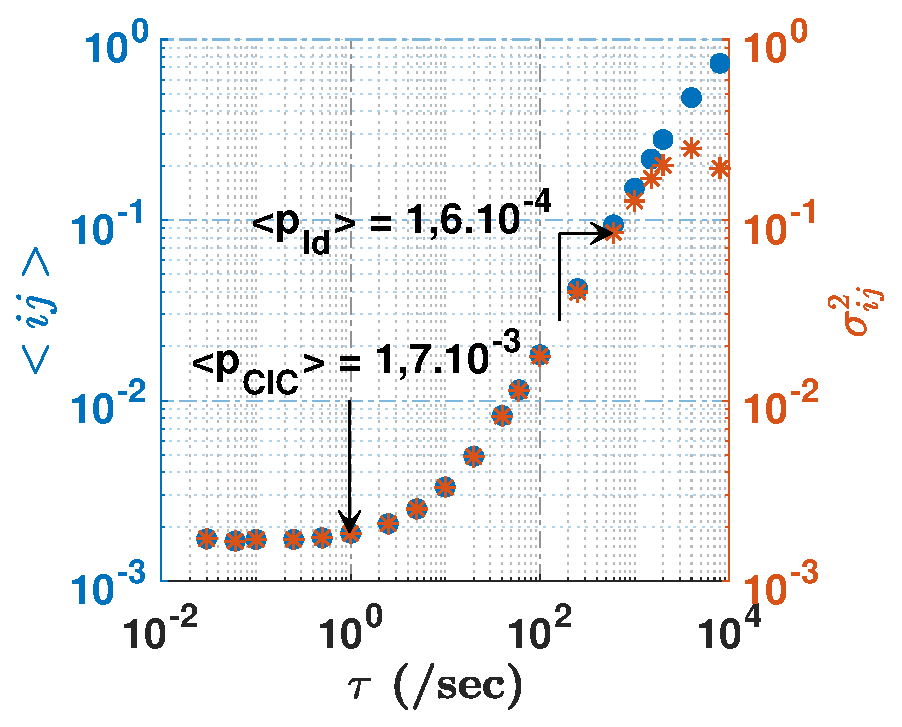
\includegraphics[width=0.40\linewidth]{fig1_caractSinglePixresponse/fig1A_meanvarIJ_Tau.eps}\label{fig:PixByPix:A}}  \\

\subfloat[]{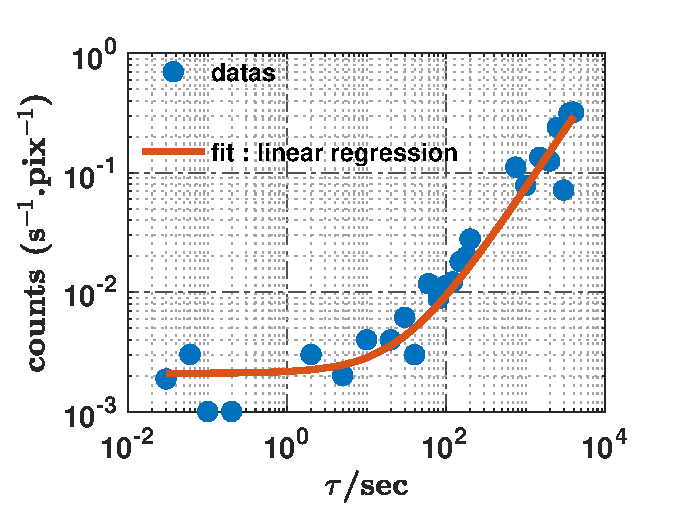
\includegraphics[width=0.40\linewidth]{fig1_caractSinglePixresponse/fig1B_fitmodel_MEF_170808_testLinFitWeighteddataPixIndex30010.eps}\label{fig:PixByPix:B}}\qquad
\subfloat[]{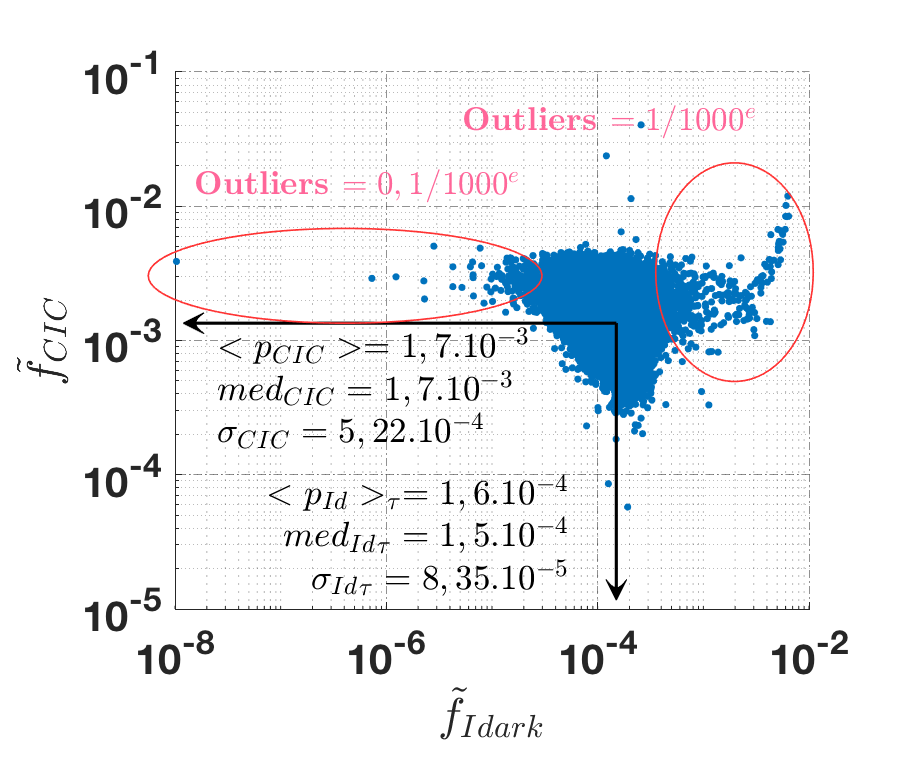
\includegraphics[width=0.4\linewidth]{fig1_caractSinglePixresponse/fig1C_PlotbiParam.eps}\label{fig:PixByPix:C}}  \\

\subfloat[]{\includegraphics[width=0.40\linewidth]{fig1_caractSinglePixresponse/fig1D_E_CumSumCIC_Python.pdf}\label{fig:PixByPix:D}} \qquad
\subfloat[]{\includegraphics[width=0.40\linewidth]{fig1_caractSinglePixresponse/fig1D_E_CumSumId_Python.pdf}\label{fig:PixByPix:E}}. \\

\subfloat[]{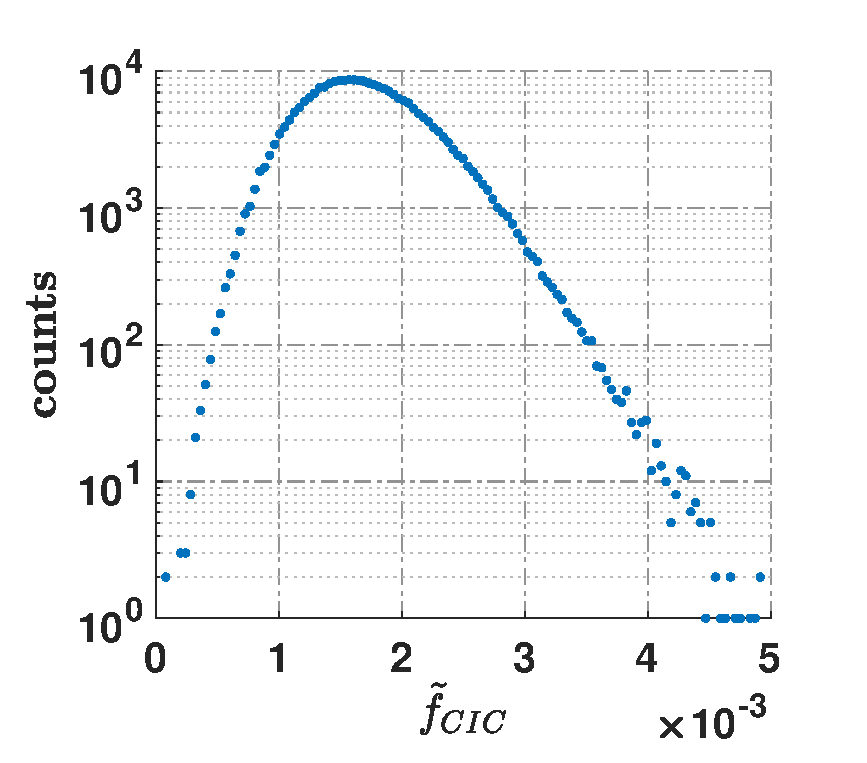
\includegraphics[width=0.35\linewidth]{fig1_caractSinglePixresponse/fig1F_G_HistoCIC.eps}\label{fig:PixByPix:F}} \qquad
\subfloat[]{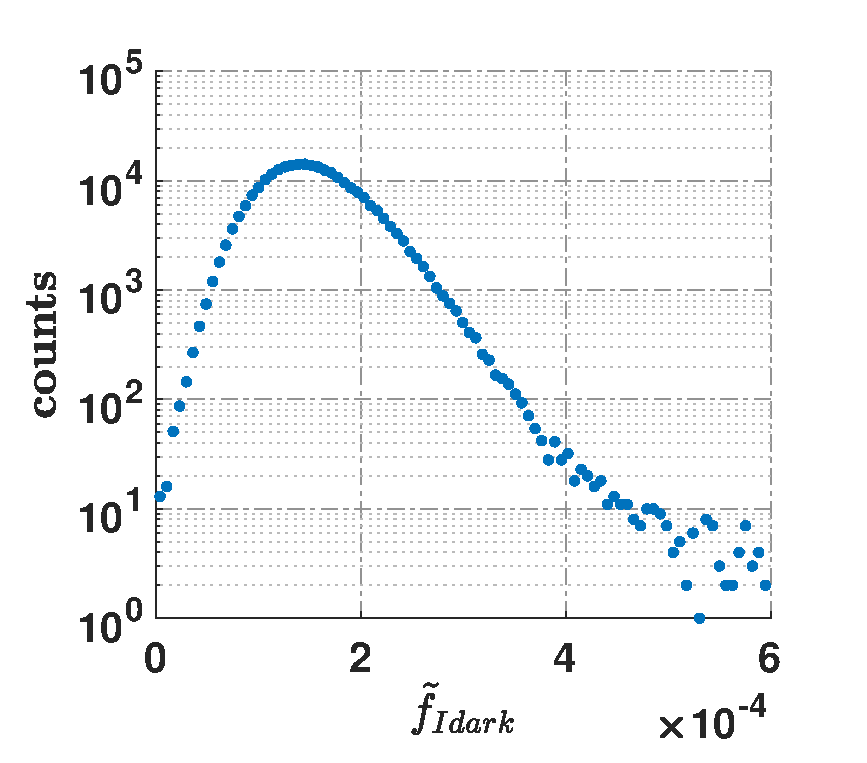
\includegraphics[width=0.35\linewidth]{fig1_caractSinglePixresponse/fig1F_G_HistoId.eps}\label{fig:PixByPix:G}} \\ 


\caption{{\bf Global detector response.} Evolution of the frequency of counts with the time of exposure  \subref{fig:PixByPix:A} .
{\bf single pixel : exemple of fit.} The individual pixel average noise response to an increased time of exposure $\tau$  was extracted and fitted out of saturation by weighted linear regression \subref{fig:PixByPix:B}. In those conditions the linear response is considered such as  <pixel$_{ij}$>$_K$$= CIC + Id * \tau$.
{\bf Caracterisation of single pixel response.} Single pixel response statistics \subref{fig:PixByPix:C}.  
Cumulative distribution (CDF) of the Clock Induced Charges (CIC) noise \subref{fig:PixByPix:D} and  the dark current (Id) \subref{fig:PixByPix:E} : Arctanh transform representation with insert in logarithmic scale  of the CDF and 1-CDF.
Histograms of the CIC \subref{fig:PixByPix:F} and the Id  \subref{fig:PixByPix:G}.}
\label{fig:PixByPix}
\end{center}
\end{figure}

\restoregeometry 



Analytically, a succession of ones and zeros has a frequency $p$ of ones and a variance $\sigma^2 = p(1-p)$ (figure \ref{fig:PoissonsIntervals:B} is a graphic representation of  $\sigma^2$ as a function of $p$ for all camera's pixels.) 
However, if this result is compatible with a pure Bernoulli, it doesn't inform about the history of pixels's counts.\par
To see if the noise of the detector is compatible with a poissonian distribution, we have to verify that the events are independents in time - history independent ; thus, we looked at the distribution of time intervalles between two pixel's count, for all pixels, and for different exposure times.(\ref{fig:PoissonsIntervals:A}.) 
As the CIC and $I_{d}$ parameters are projected on the Bernoulli parameter of the pixel for one given exposure time,  we can't extract them analytically from the fit. Also, we can't explain the factor 2 found for the fit parameter during short exposure time.  This distribution doesn't show temporal irregularities from minority pixels, fits well with an exponential function, and is therefore compatible with a truncatedPoisson distribution as described in the model. \par

Those parameters were finally integrated in our SNR model to simulate the response of our specific camera and, when used at its best, its capacity limits to detect low light fluxes.


%%!TEX root = ../ArticleCalib_main.tex
%!TEX root = ../sections/articleCalib_section4_SinglePixResponse


%%%%%%%%%%%%% FIGURE 2 BERNOUILLI POISSON INTERVALLES


\begin{figure}[htbp]
\begin{center}
\captionsetup[subfigure]{position=top, labelfont=bf, textfont=normalfont, singlelinecheck=off, justification=raggedright }

\subfloat[]{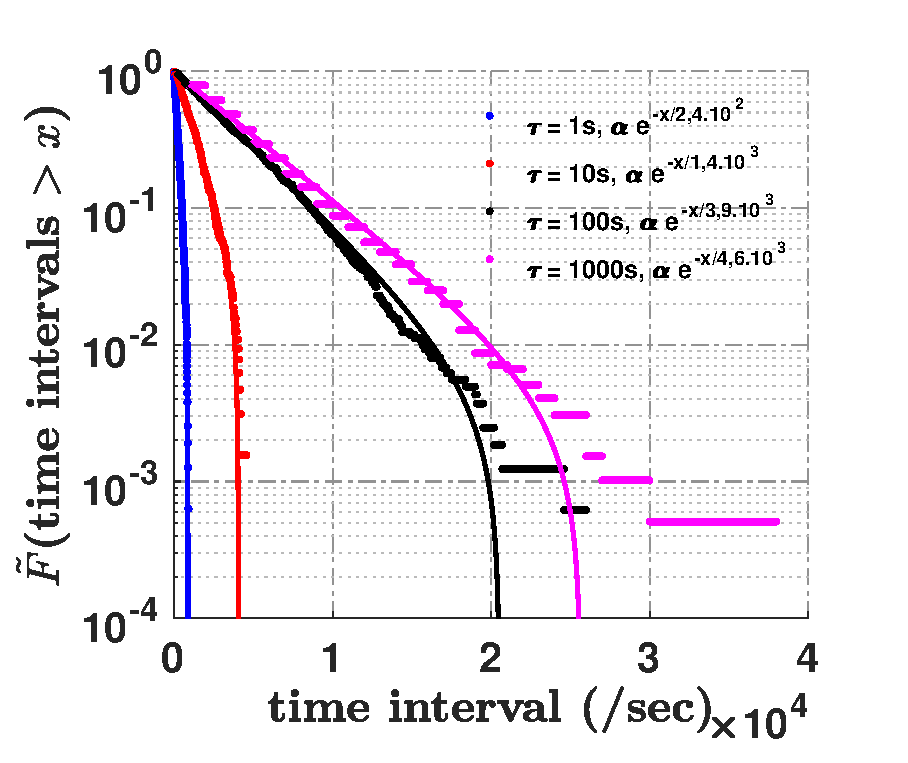
\includegraphics[width=0.4\linewidth]{fig2_ArgumentCompatiblesPoiss/fig2_Poiss_distriIntervalles.eps}\label{fig:PoissonsIntervals:A}}  
%\qquad
%\subfloat[]{\includegraphics[width=0.4\linewidth]{fig2_ArgumentCompatiblesPoiss/anlz_varmeanij_yxline_varexcess.eps}\label{fig:PoissonsIntervals:B}}  \\


\caption{{\bf Distribution of time intervals.} The complement of the cumulative distribution of the time intervals between two successive counts for a pixel$_{ij}$ for all pixels is represented. The time intervals are exctracted for differents times of exposure $\tau$ and fitted by an exponential model. For each $\tau$, the time constant found according to the model is given \subref{fig:PoissonsIntervals:A}} 
%{\bf All pixels are perfect Bernouilli.} The pixels can only take values 1 and 0. By definition they can be only fellow a  bernouilli law with  $\sigma_{ij_K}^2 = <$pixels$_{ij}>_K * (1-<$pixels$_{ij}>_K) $ strictly \subref{fig:PoissonsIntervals:B}. }

\label{fig:PoissonsIntervals}
\end{center}
\end{figure}
%%%%%%%%%%%%%%%%%%%

 	




		%!TEX root = ../ArticleCalib_main.tex
%!TEX root = ../sections/articleCalib_section4_SinglePixResponse

%%%%%%% FIGURE 1  : SINGLE PIX RESPONSE / HISTO CDF

\newgeometry{top=10mm}

\begin{figure}[]
\begin{center}
\captionsetup[subfigure]{position=top, labelfont=bf, textfont=normalfont, singlelinecheck=off, justification=raggedright }

\subfloat[]{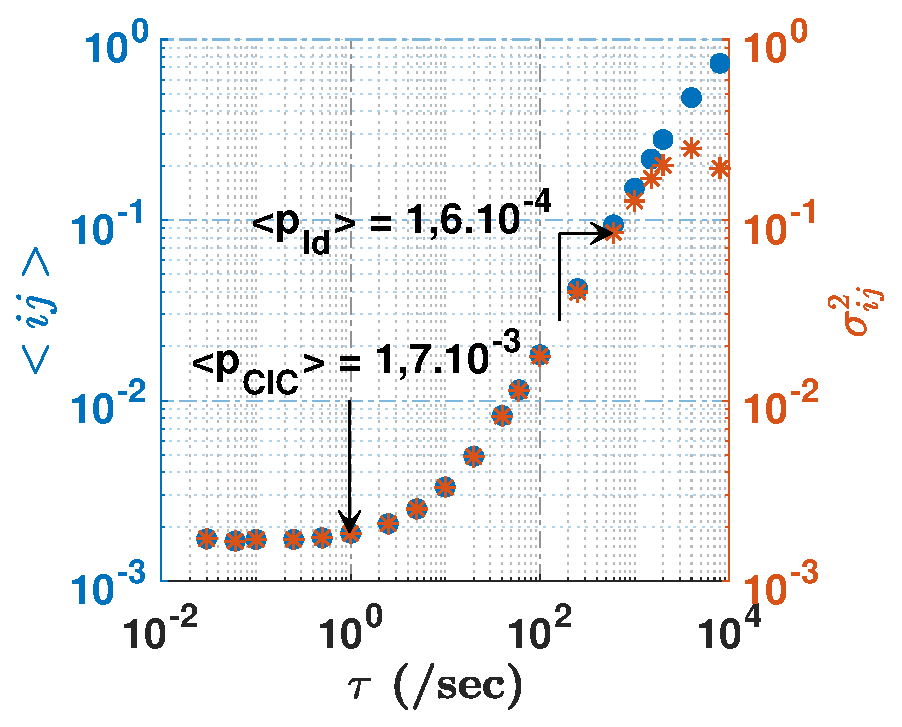
\includegraphics[width=0.40\linewidth]{fig1_caractSinglePixresponse/fig1A_meanvarIJ_Tau.eps}\label{fig:PixByPix:A}}  \\

\subfloat[]{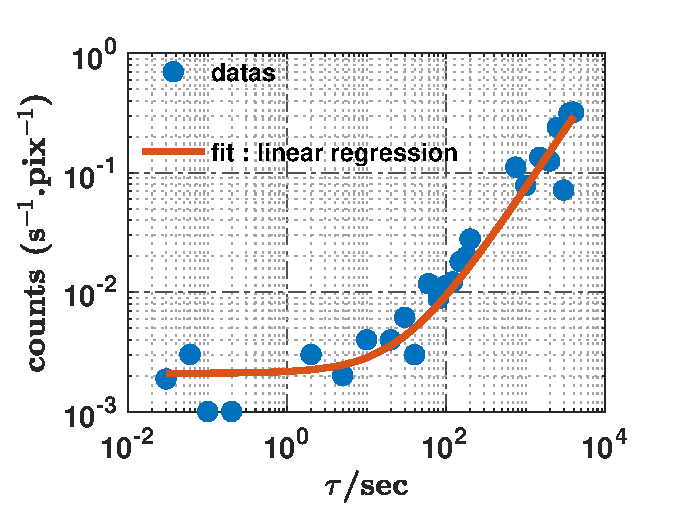
\includegraphics[width=0.40\linewidth]{fig1_caractSinglePixresponse/fig1B_fitmodel_MEF_170808_testLinFitWeighteddataPixIndex30010.eps}\label{fig:PixByPix:B}}\qquad
\subfloat[]{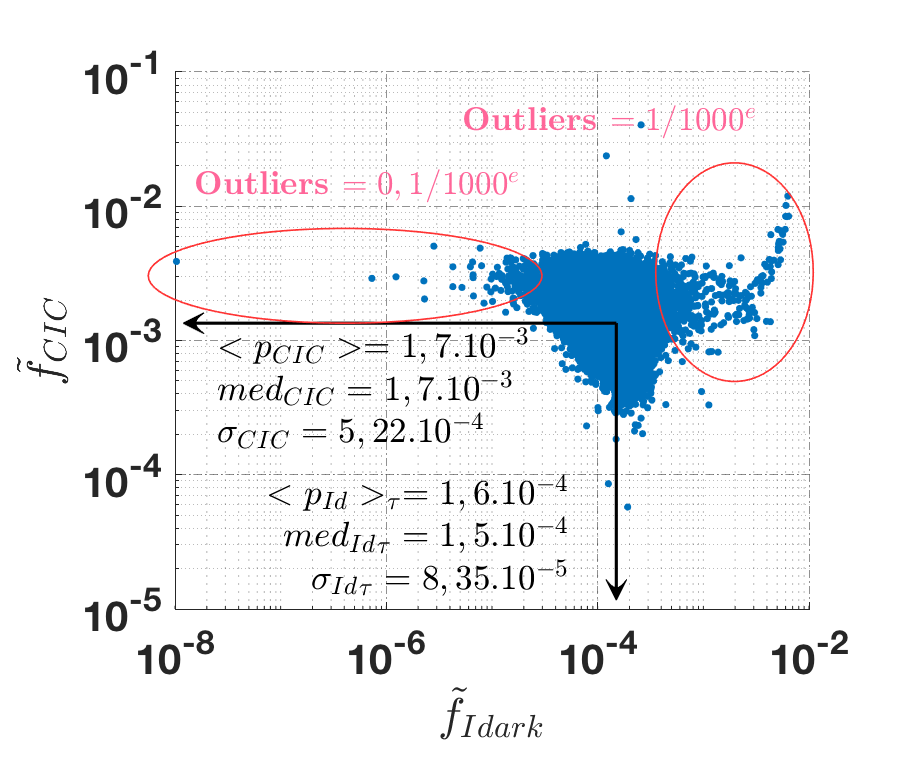
\includegraphics[width=0.4\linewidth]{fig1_caractSinglePixresponse/fig1C_PlotbiParam.eps}\label{fig:PixByPix:C}}  \\

\subfloat[]{\includegraphics[width=0.40\linewidth]{fig1_caractSinglePixresponse/fig1D_E_CumSumCIC_Python.pdf}\label{fig:PixByPix:D}} \qquad
\subfloat[]{\includegraphics[width=0.40\linewidth]{fig1_caractSinglePixresponse/fig1D_E_CumSumId_Python.pdf}\label{fig:PixByPix:E}}. \\

\subfloat[]{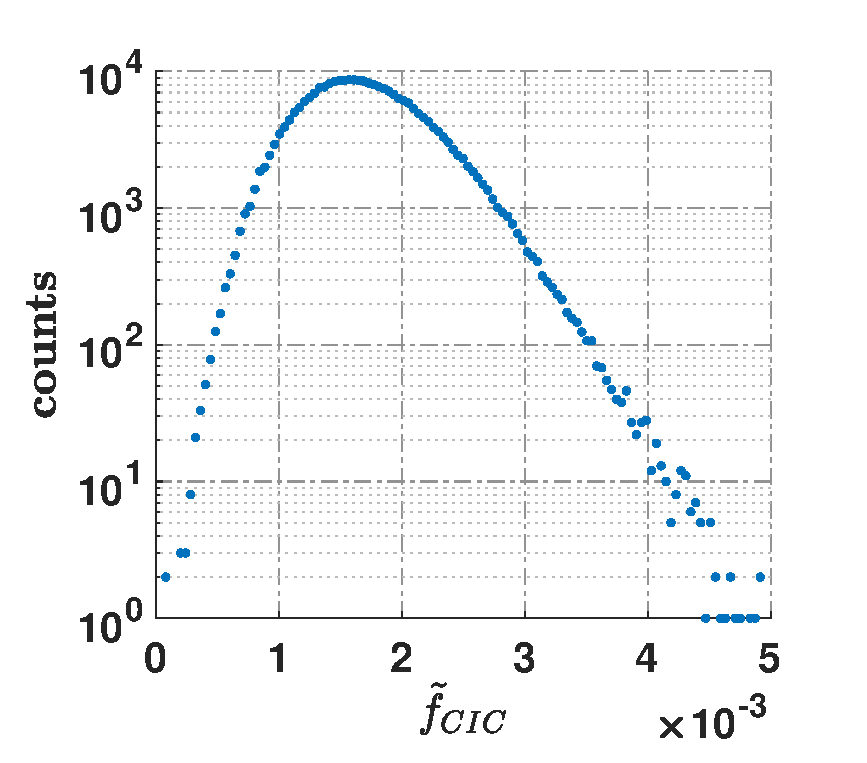
\includegraphics[width=0.35\linewidth]{fig1_caractSinglePixresponse/fig1F_G_HistoCIC.eps}\label{fig:PixByPix:F}} \qquad
\subfloat[]{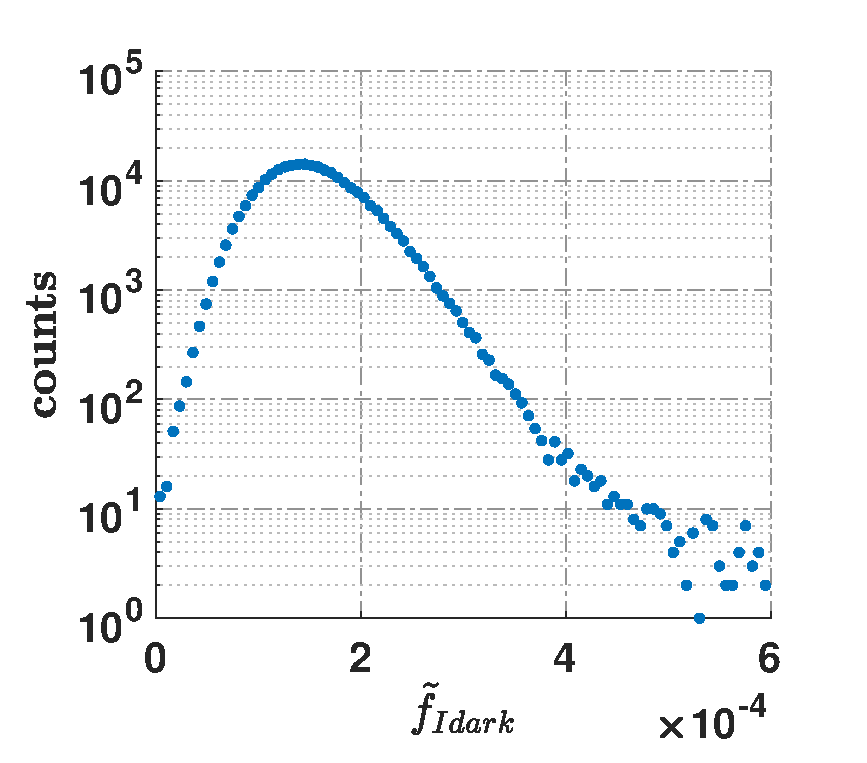
\includegraphics[width=0.35\linewidth]{fig1_caractSinglePixresponse/fig1F_G_HistoId.eps}\label{fig:PixByPix:G}} \\ 


\caption{{\bf Global detector response.} Evolution of the frequency of counts with the time of exposure  \subref{fig:PixByPix:A} .
{\bf single pixel : exemple of fit.} The individual pixel average noise response to an increased time of exposure $\tau$  was extracted and fitted out of saturation by weighted linear regression \subref{fig:PixByPix:B}. In those conditions the linear response is considered such as  <pixel$_{ij}$>$_K$$= CIC + Id * \tau$.
{\bf Caracterisation of single pixel response.} Single pixel response statistics \subref{fig:PixByPix:C}.  
Cumulative distribution (CDF) of the Clock Induced Charges (CIC) noise \subref{fig:PixByPix:D} and  the dark current (Id) \subref{fig:PixByPix:E} : Arctanh transform representation with insert in logarithmic scale  of the CDF and 1-CDF.
Histograms of the CIC \subref{fig:PixByPix:F} and the Id  \subref{fig:PixByPix:G}.}
\label{fig:PixByPix}
\end{center}
\end{figure}

\restoregeometry 

		%!TEX root = ../ArticleCalib_main.tex


%%%%%%%%%%%%% STATS MEAN COL AND LINE CIC AND IDARK

\begin{figure}[htbp]
\begin{center}
\captionsetup[subfigure]{position=top, labelfont=bf, textfont=normalfont, singlelinecheck=off, justification=raggedright }

\subfloat[]{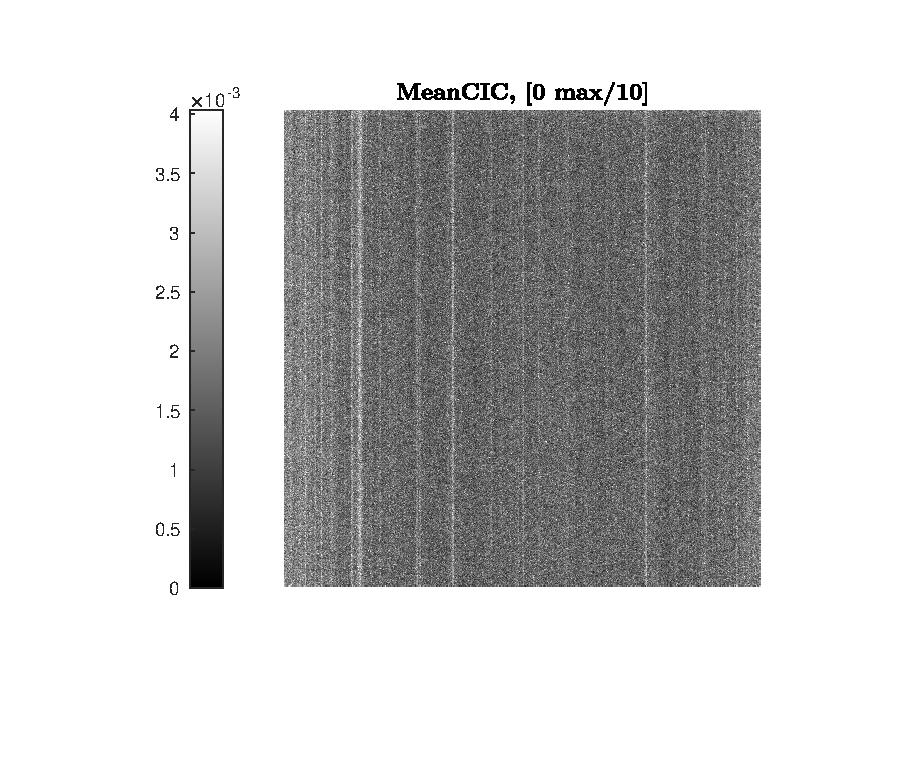
\includegraphics[width=0.49\linewidth]{fig1sup_caract_LinesColResponse/fig11Asup_ImCICmax10.eps}\label{fig:LinesColCIC:A}} \qquad
\subfloat[]{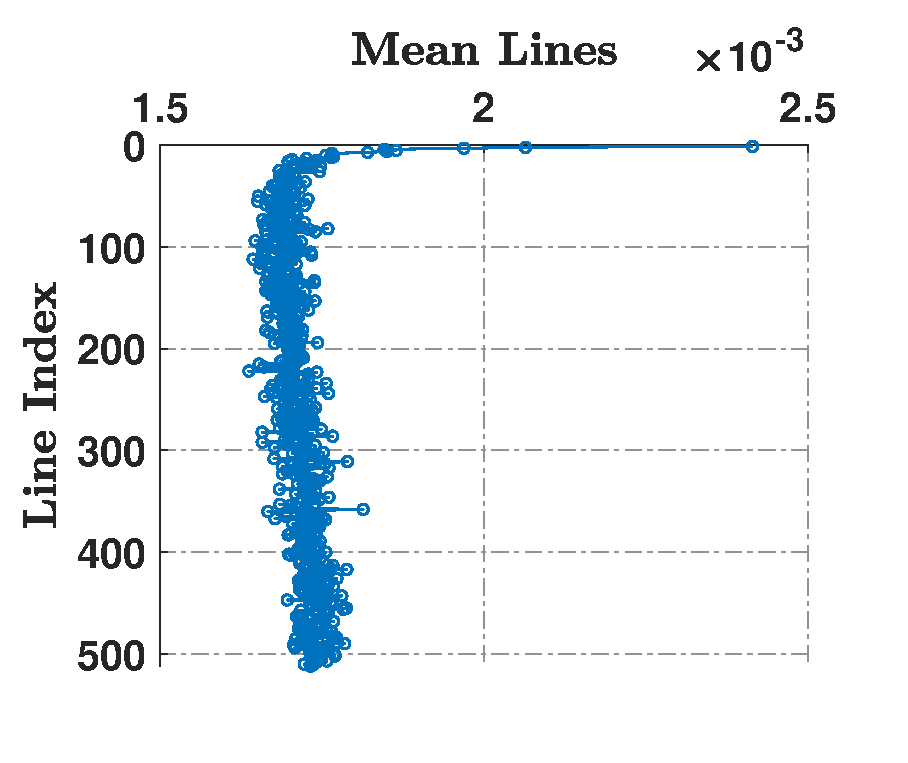
\includegraphics[width=0.4\linewidth]{fig1sup_caract_LinesColResponse/fig11Bsup_ColMean_LineMatCIC_invaxes.eps}\label{fig:LinesColCIC:B}} \\

\subfloat[]{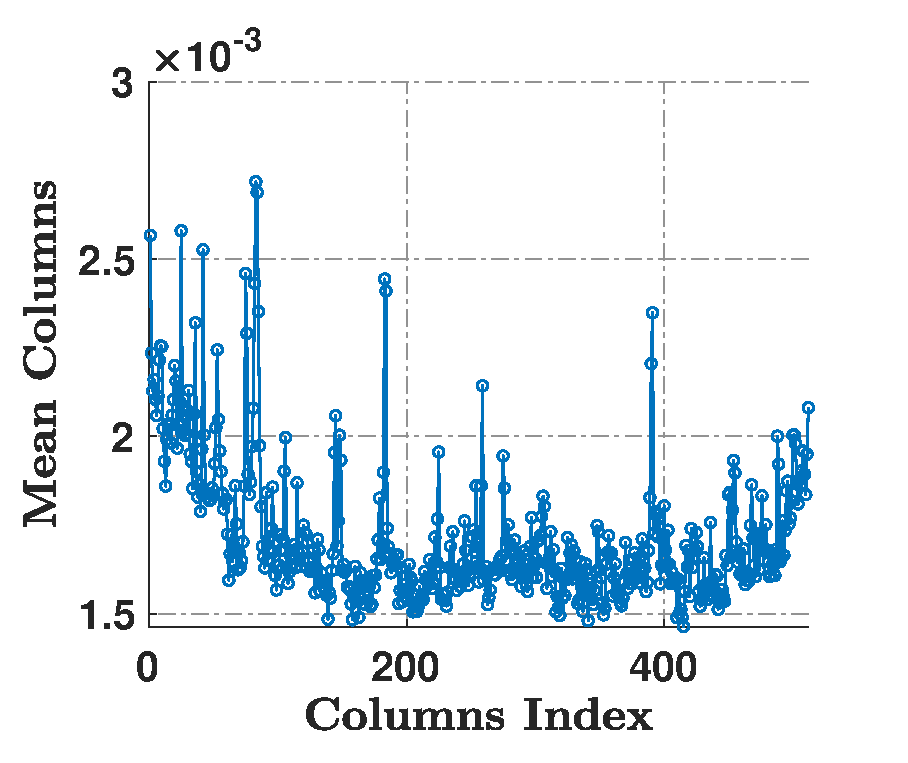
\includegraphics[width=0.4\linewidth]{fig1sup_caract_LinesColResponse/fig11Csup_RowMean_ColumnMatCIC.eps}\label{fig:LinesColCIC:C}} \qquad \qquad \qquad \qquad \qquad \qquad \qquad \qquad \qquad \qquad  



\caption{{\bf Lines and Column Pattern for CIC}.  
 Image of the CIC mean with a maximum threshold set to $1/10^e$ of the maximal pixel value.(\subref{fig:LinesColCIC:A}.)
Profile of the CIC lines (mean) (\subref{fig:LinesColCIC:B}.)
Profile of the CIC columns (mean)(\subref{fig:LinesColCIC:C}.)}
\label{fig:BBRtheo1}
\end{center}
\end{figure}


\begin{figure}[htbp]
\begin{center}
\captionsetup[subfigure]{position=top, labelfont=bf, textfont=normalfont, singlelinecheck=off, justification=raggedright }

\subfloat[]{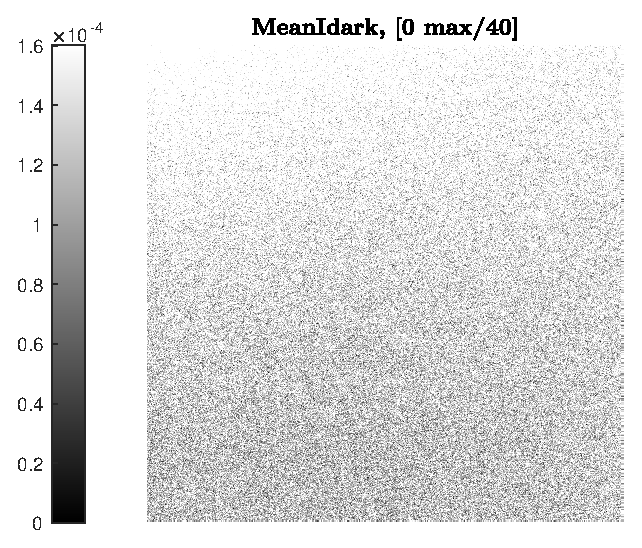
\includegraphics[width=0.35\linewidth]{fig1sup_caract_LinesColResponse/fig12Bsup_ImIdmax40.eps}\label{fig:LinesColId:A}} \qquad
\subfloat[]{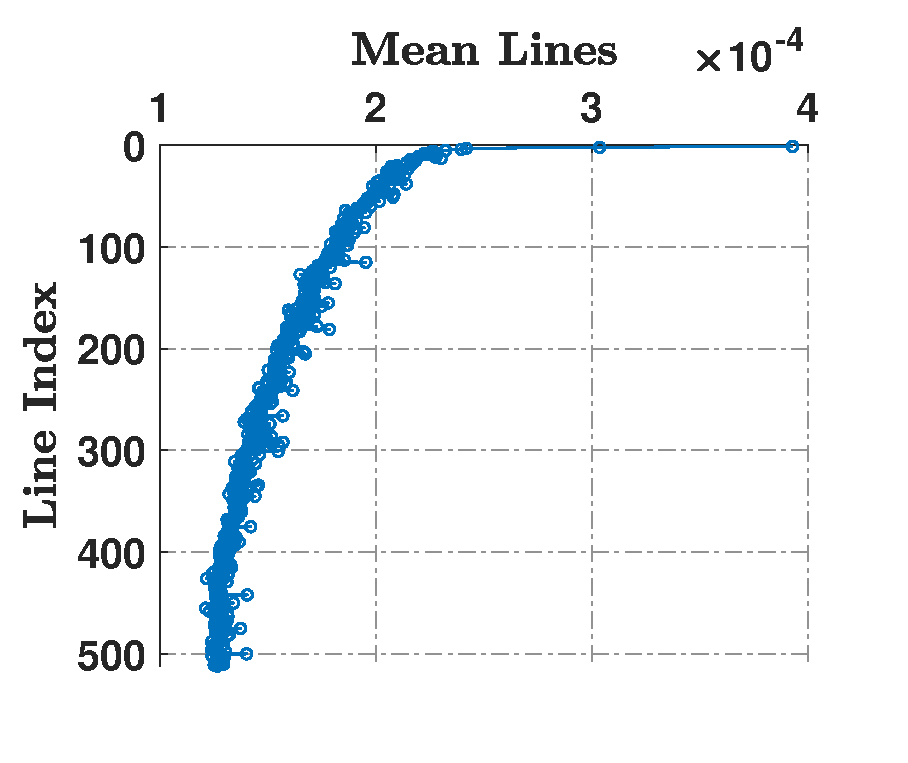
\includegraphics[width=0.4\linewidth]{fig1sup_caract_LinesColResponse/fig12Bsup_ColMean_LineMatId_invaxes.eps}\label{fig:LinesColId:B}} \\


\subfloat[]{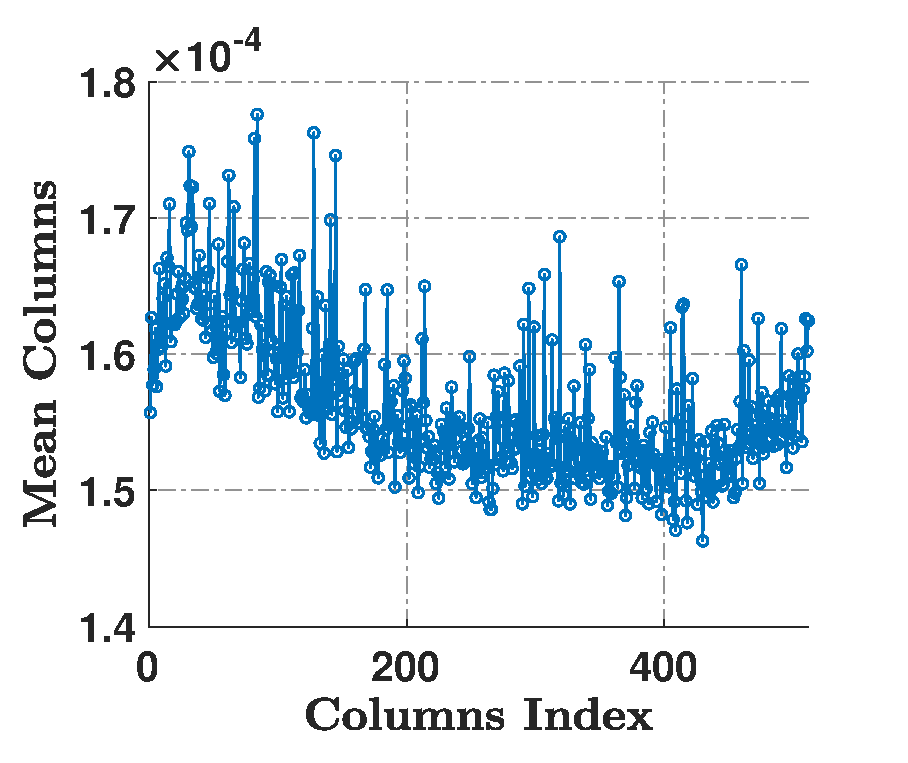
\includegraphics[width=0.4\linewidth]{fig1sup_caract_LinesColResponse/fig12Csup_RowMean_ColumnMatId.eps}\label{fig:LinesColId:C}} \qquad
\subfloat[]{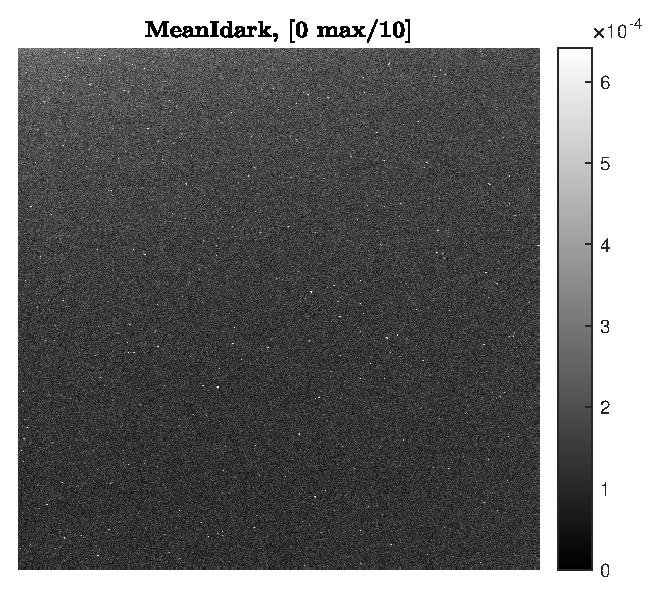
\includegraphics[width=0.35\linewidth]{fig1sup_caract_LinesColResponse/fig12Asup_ImIdmax10.eps}\label{fig:LinesColId:D}} 



\caption{{\bf Lines and Column Pattern for Id}.  
  Image of the Id mean with a maximum threshold set to $1/40^e$ of the maximal pixel value.(\subref{fig:LinesColId:A}.)
  Profile of the Id lines (mean) (\subref{fig:LinesColId:B}.)
  Profile of the Id columns (mean) (\subref{fig:LinesColId:C}.)
  Image of the Id mean with a maximum threshold set to $1/10^e$ of the maximal pixel value.(\subref{fig:LinesColId:D}.)}
\label{fig:BBRtheo1}
\end{center}
\end{figure}


		%!TEX root = ../ArticleCalib_main.tex
%!TEX root = ../sections/articleCalib_section4_SinglePixResponse


%%%%%%%%%%%%% FIGURE 2 BERNOUILLI POISSON INTERVALLES


\begin{figure}[htbp]
\begin{center}
\captionsetup[subfigure]{position=top, labelfont=bf, textfont=normalfont, singlelinecheck=off, justification=raggedright }

\subfloat[]{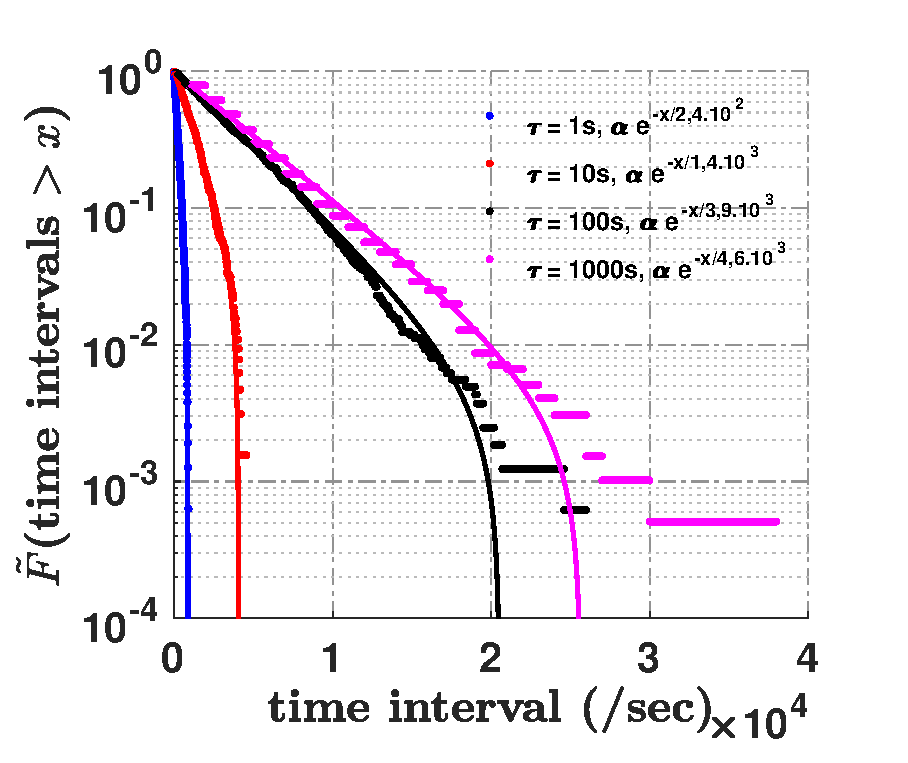
\includegraphics[width=0.4\linewidth]{fig2_ArgumentCompatiblesPoiss/fig2_Poiss_distriIntervalles.eps}\label{fig:PoissonsIntervals:A}}  
%\qquad
%\subfloat[]{\includegraphics[width=0.4\linewidth]{fig2_ArgumentCompatiblesPoiss/anlz_varmeanij_yxline_varexcess.eps}\label{fig:PoissonsIntervals:B}}  \\


\caption{{\bf Distribution of time intervals.} The complement of the cumulative distribution of the time intervals between two successive counts for a pixel$_{ij}$ for all pixels is represented. The time intervals are exctracted for differents times of exposure $\tau$ and fitted by an exponential model. For each $\tau$, the time constant found according to the model is given \subref{fig:PoissonsIntervals:A}} 
%{\bf All pixels are perfect Bernouilli.} The pixels can only take values 1 and 0. By definition they can be only fellow a  bernouilli law with  $\sigma_{ij_K}^2 = <$pixels$_{ij}>_K * (1-<$pixels$_{ij}>_K) $ strictly \subref{fig:PoissonsIntervals:B}. }

\label{fig:PoissonsIntervals}
\end{center}
\end{figure}
%%%%%%%%%%%%%%%%%%%

 	
	
%%%%%% SIMULATION RESULTS
	%%!TEX root = ../ArticleCalib_main.tex

%%%%%%% SIMULATION article calib
\section{Simulation results and SNR}

The simulation of the camera shows the expected total number of counts on the detector N1 and its variance  under different uniform and constant light fluxes. The signal is competing with the dark current when the exposure time increases, hence the incident light flux is expressed by a fraction $\epsilon $ of the dark current flux equivalent. When the time of exposure increases, the N1 mean reaches a maximum (ie. the total number of functional pixels : 512$\times$512) (\ref{fig:SimuMeanVarN1:A}) and the N1 variance increases and then collapses to stabilise at a minimum (\ref{fig:SimuMeanVarN1:B}). \par

Because of the dynamics linked to the saturation, the SNR presents a maximum, before diminishing with the exposure time.
For fluxes that exceed $I_{d}$ flux equivalent, a "bump" appears at the top of SNR curves : when approaching saturation, i.e. when the Bernoulli probability approaches $1$, the distribution is somehow "compressed", and the variance decreases while the mean still increases(\ref{fig:SNRTau:A}.)
	
		%!TEX root = ../ArticleCalib_main.tex

%%%%%%%%%%%%% FIGURE 3 FIT MODEL 


\begin{figure}[htbp]
\begin{center}
\captionsetup[subfigure]{position=top, labelfont=bf, textfont=normalfont, singlelinecheck=off}

\subfloat[]{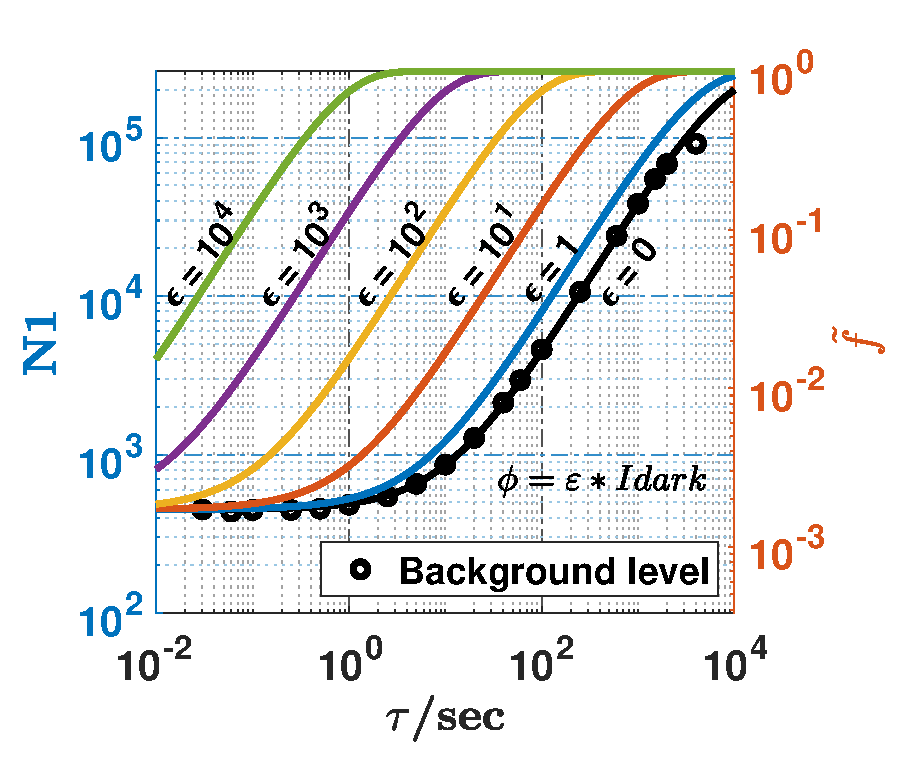
\includegraphics[width=0.4\linewidth]{fig3_model_fit/fig3A_fitmodel_ModelHeterogenN1Tau_dataTau.eps}\label{fig:SimuMeanVarN1:A}}  \qquad
\medskip
\subfloat[]{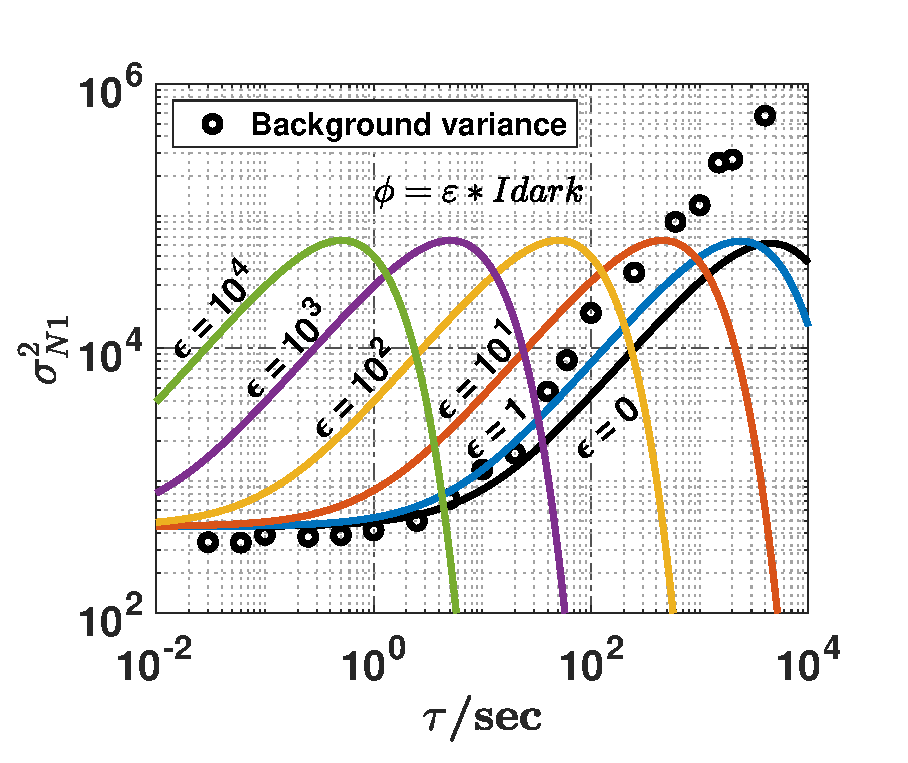
\includegraphics[width=0.4\linewidth]{fig3_model_fit/fig3B_fitmodel_ModelHeterogenVarN1Tau_TauData.eps}\label{fig:SimuMeanVarN1:B}} \qquad


\caption{{\bf wide detector response : simulation and data.}  The model  gives the simulation of the wide detector response N1 (N1 = $\sum_{ij}$pixels) \subref{fig:SimuMeanVarN1:A} and its variance  \subref{fig:SimuMeanVarN1:B} for different fluxes. The experimental noise (N1) and its variance are represented.}
\label{fig:SimuMeanVarN1}
\end{center}
\end{figure}
%%%%%%%%%%%%%%%%%%%



	
%%%%%% CONSTANT, UNIFORM FLUX MEASUREMENT STRATEGY
	%%!TEX root = ../ArticleCalib_main.tex

%%%%%%% CONSTANT, UNIFORM FLUX MEASUREMENT STRATEGY article calib
\section{Constant, Uniform light flux measurement strategy}

The SNR per frame presenting a maximum suggests an existing optimal strategy, ie an optimal time of exposure, for a given light flux intensity, under the conditions of acquisition described - gain 3000, PC mode, -85°c chilling. \par

Using a SNR contour representation permits a graphical approach to predict our single frame detection capacity, of a given light flux, for a given exposure time  (\ref{fig:SNRTau:B}). For exemple, with 40 photons/cm$^2$/sec (Id equivalent), the SNR equal 1, for one acquisition of 1 second exposure time.\par
\medskip


Going further, on the figure \ref{fig:SNRTau:A}}, we observe two main SNR regimes that can be defined as a function of their logarithmic slope. One fellows a logarithmic slope of 1 ("regime 1"), and the other  fellows a logarithmic slope of $1/2$ ("regime $1/2$"). \par

Hence, the fellowing question : should we repeat the same acquisition K times during the total experimentation time t, or should we fix $t = \tau$ if $t < \tau_{SNR max}$ ?
Studying those SNR regimes will helps us to answer this question.\par

Indeed, the SNR increases with the number of repetition of acquisitions K in the same experimental conditions, given that the standard error of the mean (SEM) decreases with $\sqrt{K}$, and with the time of exposure $\tau$, until it reaches the time for which the SNR is maximal $\tau_{SNR max}$.
In the "regime 1", the SNR increases proportionally to $\tau$ and to $\sqrt{K}$, while in the "regime $1/2$", the SNR increases proportionally to $\sqrt{\tau}$ and to $\sqrt{K}$.
Therefore, considering one flux intensity $\phi$ and time of exposure $\tau$, in "regime 1", the SNR increases faster with $\tau$ than with K, whereas in "regime $1/2$", the SNR increases indifferently  with $\tau$ and with K.\par

Those regimes are better viewed with the logarithmic derivative $\delta logSNR / \delta log\tau$ representation (\ref{fig:SNRTau:C}).
Here, we noticed that there is only one precise $\tau$ for which the logarithmic derivative of the SNR takes the value $1/2$, and this $\tau$ stands for the "regime $1/2$".
Below this time of exposure, increasing the $\tau$ increases the SNR faster than increasing K ; above it, increasing the K increases the SNR faster than increasing  $\tau$. But, repeating an acquisition at the precise time of exposure where $\delta logSNR / \delta log\tau = 1/2$ brings the maximum increasing rate of the SNR once passed the "regime 1".
Therefore we called this new characteristic time of exposure the  $\tau$ of maximal density information ($\tau_{max \hspace{3} info}$).\par
\medskip


From this analysis, two characteristic exposure times are extracted : $\tau_{SNR max}$ gives the maximum SNR for one frame, and the $\tau_{max \hspace{3} info}$ gives the best information density when repeated, both dependant on known or predicted incident light fluxes.
In practice, for a long detection of a flux intensity near the dark current level, an repeated exposure time around $500-600$ sec is best, while for an inferior flux intensity, the ideal repeated exposure time is slightly higher, around $700-800$ sec.
This deep study gives us a great tool to use our detector at its best, but also to predict our detection capacity for one uniform, constant light flux emitting source or sample (\ref{fig:SNRTau:D}.)\par   

However other kind of unpredicted fluctuations can impair the model (\ref{fig:SimuMeanVarN1:B} shows N1 variance excess). Thus, improving experimentally the SNR by a better light collection, and having a \textit{in situ} control with imaging, is also fondamental in ultra weak light flux detection.  










 (\ref{fig:SNRTau:B}). 
	
		%!TEX root = ../ArticleCalib_main.tex

%%%%%%%%%%%%% FIGURE 4 : SNR / TAU OPTIMAL SEGMENTATION


\begin{figure}[htbp]
\begin{center}
\captionsetup[subfigure]{position=top, labelfont=bf, textfont=normalfont, singlelinecheck=off, justification=raggedright }

\subfloat[]{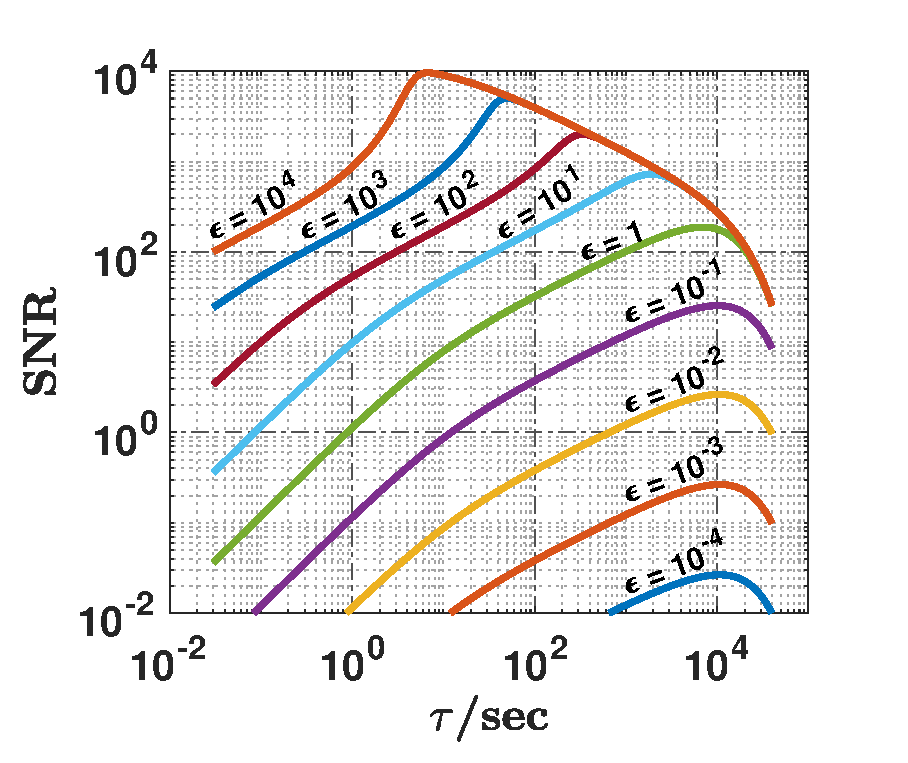
\includegraphics[width=0.4\linewidth]{fig4_model_segmentation/fig4A_SNRtau.eps}\label{fig:SNRTau:A}}  \qquad
\subfloat[]{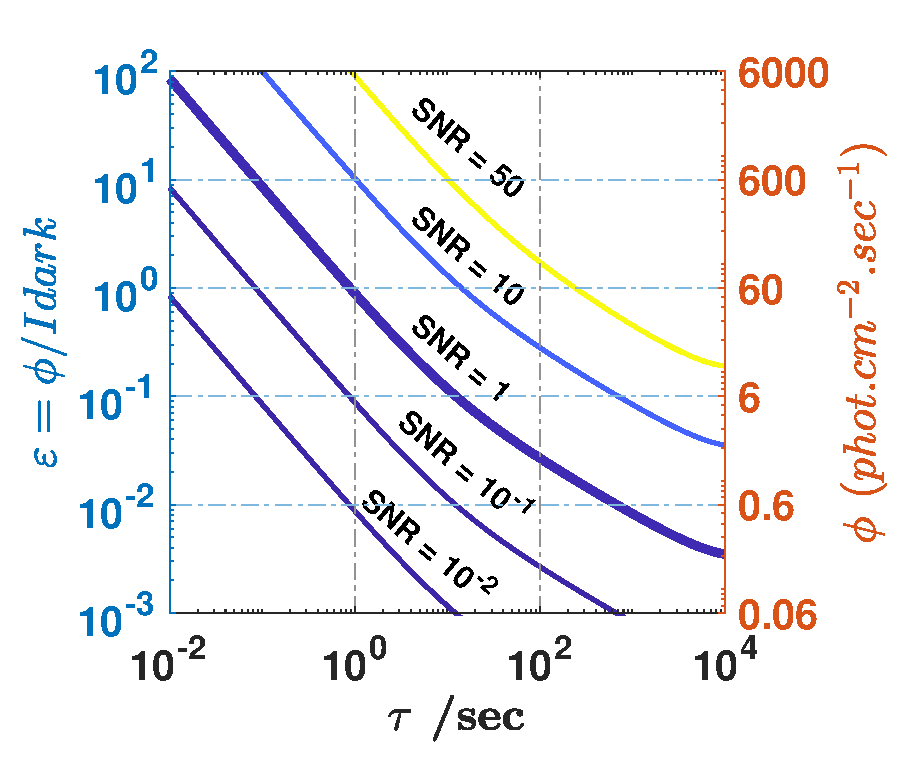
\includegraphics[width=0.4\linewidth]{fig4_model_segmentation/fig4B_SNRcontour.eps}\label{fig:SNRTau:B}}  \\

\subfloat[]{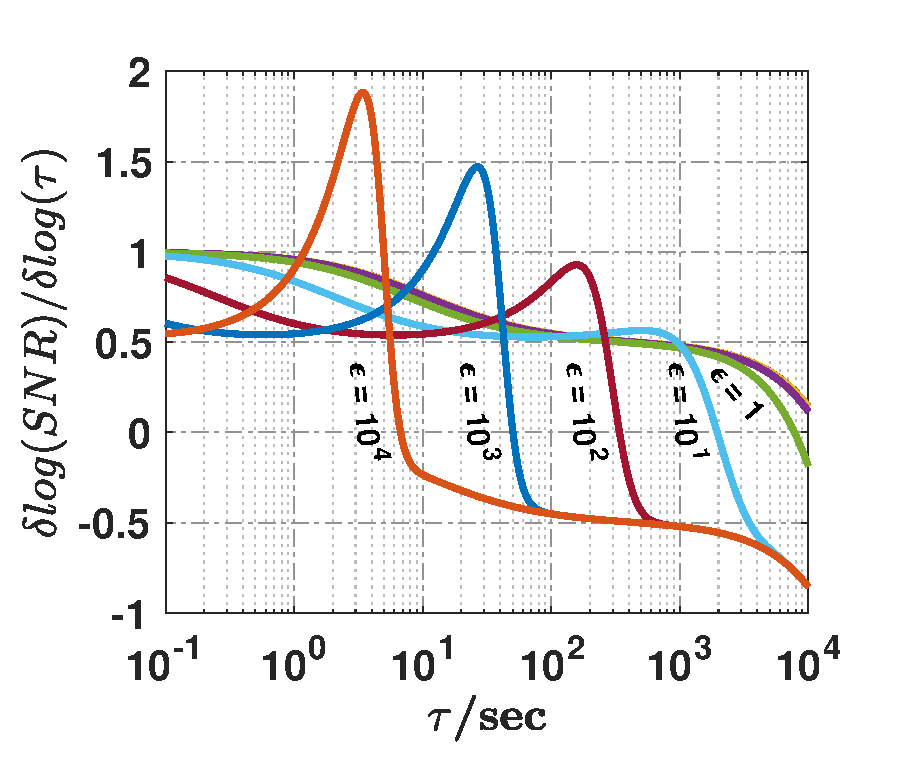
\includegraphics[width=0.4\linewidth]{fig4_model_segmentation/fig4C_derivelogSNRTau.eps}\label{fig:SNRTau:C}} \qquad
\subfloat[]{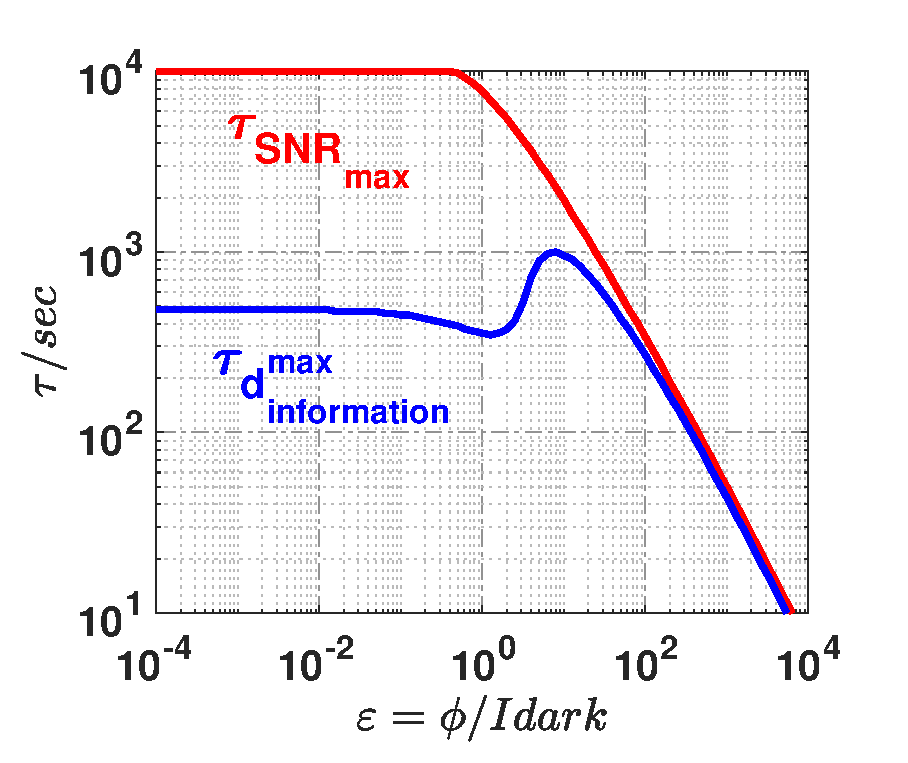
\includegraphics[width=0.4\linewidth]{fig4_model_segmentation/fig4D_SNRtaudensitemax_snrmax.eps}\label{fig:SNRTau:D}}. \\


\caption{{\bf SNR simulation.} The SNR simulation is represented for different fluxes $\phi$ expressed as a fraction $\epsilon$ of the dark current Id. The x axes is extended to $10^5$ seconds to show the effect of the saturation on the SNR in photon counting mode \subref{fig:SNRTau:A}. Figure  \subref{fig:SNRTau:B} shows the corresponding SNR contour plot.
{\bf What is the optimal time of exposure.}  Figure \subref{fig:SNRTau:C} shows the logarithmic derivative of the SNR ($\delta logSNR/\delta log\tau$) for different fluxes. The time of maximal information density ($\tau_{d_{info}^{max}}$) is such as  $\delta logSNR/\delta log\tau = 0,5$  \subref{fig:SNRTau:D}. The time of maximal SNR  ($\tau_{SNR^{max}}$) is comparatively represented. }
\label{fig:SNRTau}
\end{center}
\end{figure}
%%%%%%%%%%%%%%%%%%%



		
%%%%%% FLUCTUATING FLUX MEASUREMENT ?
	%%!TEX root = ../ArticleCalib_main.tex

%%%%%% FLUCTUATING OR HETEREGONEOUS FLUX MEASUREMENT ? article calib
\section{Fluctuating light flux and heterogeneous emission}

The measure of a fluctuating light flux implies a statistic filtration to detect a double stochasticity.
In other words, when sampling the acquisition, do the fluctuations exceed the expected stochastic fluctuations of the observable ?
If the exposure time is larger than the fluctuation period, we won't determine if there are signal variations, whereas if the exposure time is smaller than the fluctuation period, but the signal is too weak to achieve a sufficient SNR per frame, or by repeating frames, we won't determine if there is a signal at all. \par
Hence, there is a time resolution limit for a given light flux, depending on the minimal time of exposure to be repeated or to be met to have a sufficient SNR, compared to the variation period and amplitude of the signal.\par
\medskip


To image an object emitting an heterogeneous light flux, we have to address the question in part \ref{sec:SinglePixCaract} :  is a pattern of pixels consistent with the random effect of a perfectly uniform optical field, or is it produced by a contrasted object ? Knowing perfectly the background of each pixels for a given exposure time permits to do tests of spatial randomness to detect an non uniform light field on the detector. A pixel by pixel study is less sensible than a hole detector detection as it will rely uniquely on the number of repetitions of frames to make a significative difference in between pixels. \par
If we know the image position on the captor, and if the image light flux is uniform, the strategy can be different : to increase the detection sensibility, we can then sum all pixels of the background area and the lit area, as we did for the entire detector, and compare and quantify both observables.\par
Combining methods as per fit is one's strategic choice to make.






					
		
%%%%%% PRACTICALLY
	%%!TEX root = ../ArticleCalib_main.tex

%%%%%% FLUCTUATING OR HETEREGONEOUS FLUX MEASUREMENT ? article calib
\section{Practically}

We address here different practical issues or questions about fast SNR simulation, cosmic rays, and and thermal radiation detection

%% Fast SNR simulation
\subsection{Fast SNR simulation}

Taking into account the 513$\times$512 pixels into a sum of Bernoulli random variable with their own parameter is time consuming, and for the single pixel characterisation, and for the simulation processing. 
If a subtle knowledge of the camera pixels is not necessary, estimating the SNR by a model is swiftly done by considering the detector homogeneous, with the same CIC and Id parameter for all pixels. The parameters are extracted by doing a simple linear regression ($\tilde{f_{counts}} = \tilde{f_{CIC}} + \tilde{f_{Id}}*\tau$) out of saturation on the global detector response on complete dark conditions (see \ref{fig:PixByPix:A}).\par
The difference between both homogeneous model (all pixels's noises identical), and the heterogeneous model (all pixels's noises singular), is the variance between pixels on one frame, $\sigma^2_{ij}$. Surprisingly enough, this $\sigma^2_{ij}$ is subtracted to the N1 variance in the heterogeneous model case, which leads to a better SNR (\ref{fig:SNRTau:HeteroHomo}). 
It is easily demonstrated by :   \par

\textcolor{blue}{demonstration de la difference}.\par
\medskip
However, the difference is small enough (from 1 to 7\%) for neglecting it for the sake of simplicity. 
%
	%\input{figures/articleCalib_fig4supp_model_HeteroHomo}
	
%% Cosmic rays
\subsection{Cosmic rays}

Cosmic rays (CR) are particles of different kinds, carrying a wide range of energies. They arrive from the cosmos and trigger multipixel response patterns on the detector (see \ref{fig:CR:A}). 
Because these pixel clusters patterns bear some reproducible features (a cluster of connected pixels followed by a "horizontal tail"), we wrote a program to detect a given number of connected pixels, this cut off number of connected pixels being determined by a negligible probability ($<10^{-6}$) to happen randomly for a given time of exposure. The frequency of events (ie. cluster of connected pixels), as function of the number of pixels in the cluster, was determined by a Monte Carlo simulation, on an arbitrary large enough detector to achieve sufficient statistic, using our model to produce the noise pattern, for different time of exposure. This program create a detector equivalent logical matrix attributing "ones" to the pixels belonging to a cluster's size bigger than the determined cut off. After indexing the concerned pixels, we substitute them by random values drawn from the appropriate Bernoulli distribution.
Because the detection of these clusters relies on the recognition of connected pixels, it becomes more difficult to tell them from clusters generated by signal photons when the density of positive pixels is too high, e.g. when the time of exposure exceeds 2000 seconds. 
However, we could assess the contribution of cosmic rays and we found that, in photon counting mode, it amounts to $4,1.10^{-6}$ electrons/sec/pixels, that is $1/20$ of the dark current (figures \ref{fig:CR:B} and  \ref{fig:CR:C}.) \par

Importantly, this equivalence with an effective photon rate determined in binary mode (photon counting) is physically meaningless, because it does not reflect the actual strength of cosmic rays which saturate analog detectors.
Digital treatment makes these high energy perturbations look like regular visible photons, and this can be considered as an additional advantage of using a binary mode to detect low light fluxes. \par
We consider that the impact of the cosmic ray on our model is negligible, as far as the concerned time of exposure are small enough that their removal doesn't impact significantly the statistic of the wide detector response.\par
%
	%\input{figures/articleCalib_Fig5_CR}


%% BBR
\subsection{Black Body Radiation}

Given the SNR model a rightful question emerged : what is the sensitivity of our camera to thermal radiation ? Indeed, the signal of interest being so weak, it is fundamental to be able to distinguish it from other kind of radiation and fluctuation linked to temperature. This is even more crucial given that we aim for biological sample that are kept at higher temperature (37 celsius degrees) than room temperature.\par
%During extensive measures trying to uncover the origin of N1 outliers, we noticed significant fluctuations happening in the background noise producing a double stochasticity effect.
%We went further by measuring directly the thermal flux with the help of a Black Body and we realised that we were sensitive to changes of temperature (see figure \ref{fig:BBR:exp_100s_600s}). 

Therefore, we modelled the sensitivity of our detector to temperature changes, considering its spectral sensitivity (see figure \ref{fig:BBR:NuvuQESpectra}), and the black body radiation spectra (\ref{fig:BBRtheo1:A}.). \par
Our detector is indeed sensitive to temperature, according to the model, and in a much more drastic way that we expected.  Given a time of exposure of 600 sec, the SNR is 10 and 100 (according to our SNR model (see figure \ref{fig:SNRTau:B}) for the thermal flux given at a temperature of  23-25c and 37-38c respectively. The saturation of the detector happens for 58\°c ( see figure \ref{fig:BBRtheo1:C}). The Noise Equivalent Temperature Difference (NETD) for a thermal flux given at temperatures 20c, 26c, 32c and 37c is respectively 2, 1, 0.5, 0.2 (figure \ref{fig:BBRtheo2}).\par
It means that for a sample maintained at 37c, the camera would be sensitive to  a 0.2c change of temperature. It shows that the measured level of our background for a given $\tau$ is actually temperature dependent.  \par
This very recent result raises new challenges for temperature and environment control that are for now unprecedented and was never considered in this field.\par

%	
	%\input{figures/articleCalib_fig6_BBRtheocalibration}


	
		%!TEX root = ../ArticleCalib_main.tex

%%%%%%%%%%%%% FIGURE 5 : SNR / MODEL HETERO/HOMOG


\begin{figure}[htbp]
\begin{center}
\captionsetup[subfigure]{position=top, labelfont=bf, textfont=normalfont, singlelinecheck=off, justification=raggedright }

\subfloat[]{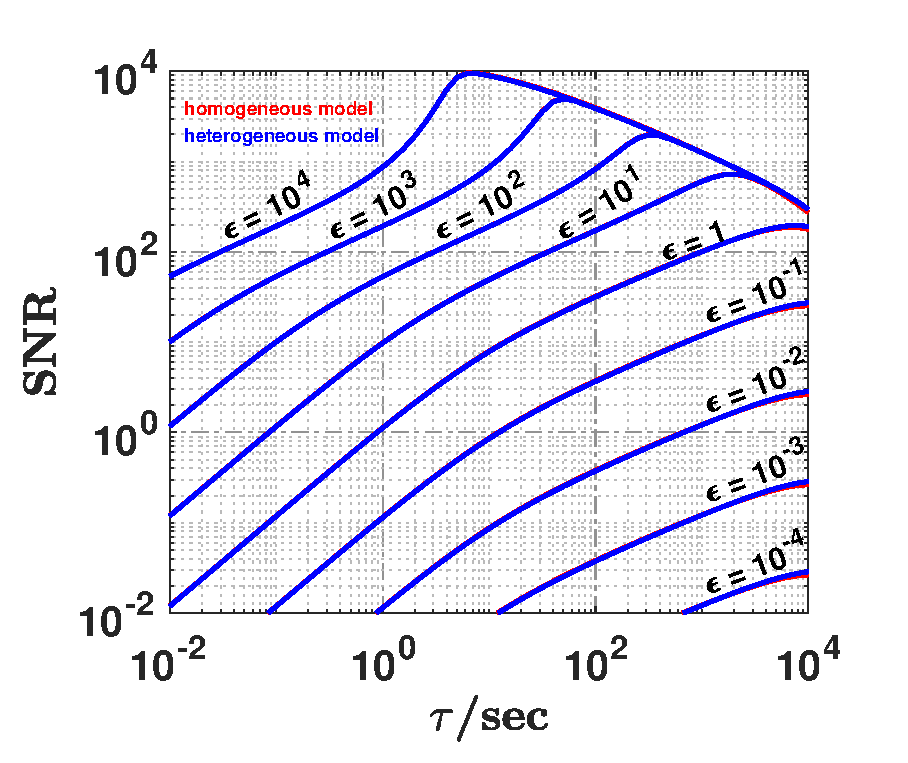
\includegraphics[width=0.4\linewidth]{fig5_compHomoHetero/fig5A_NuvuSimu_E_SNRTau_comparaisonHeteroHomo.eps}\label{fig:SNRTau:HeteroHomo:A}}  \qquad
\subfloat[]{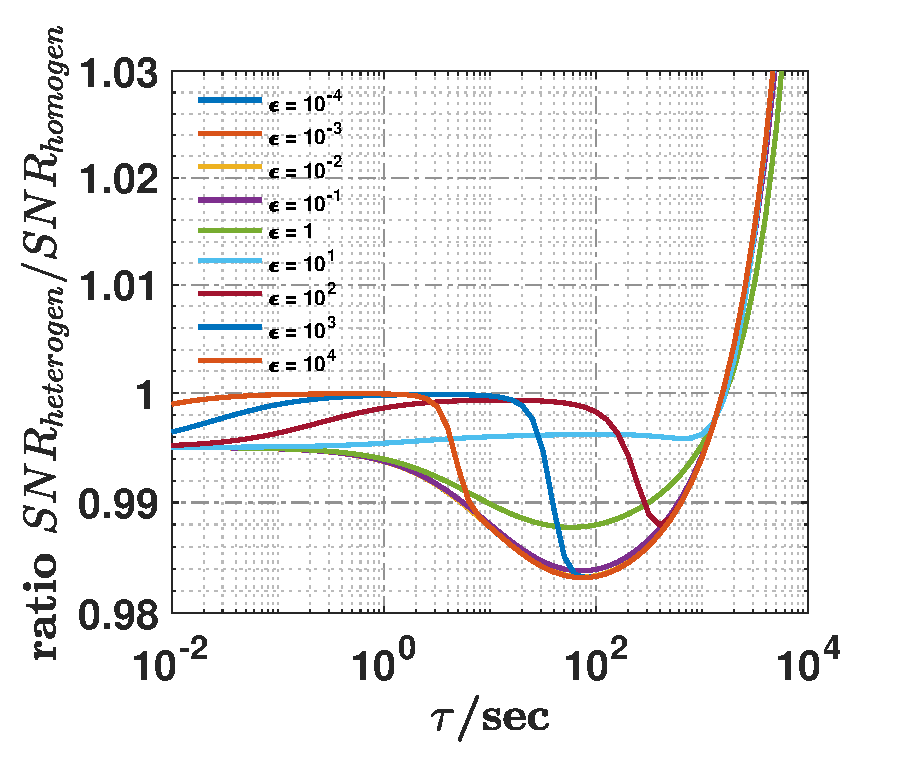
\includegraphics[width=0.4\linewidth]{fig5_compHomoHetero/fig5B_SNR_NuvuSimu_E_SNRTau_ratioHeteroHomo.eps}\label{fig:SNRTau:HeteroHomo:B}}  \qquad


\caption{{\bf SNR models comparaison.} The SNR simulation is represented for different fluxes $\phi$ expressed as a fraction $\epsilon$ of the dark current Id for both the heterogeneous and homogeneous model (\subref{fig:SNRTau:HeteroHomo:A}). The ratio between the SNR for the heterogeneous and homogeneous model is presented in figure \subref{fig:SNRTau:HeteroHomo:B}. }
\label{fig:SNRTau:HeteroHomo}
\end{center}
\end{figure}
%%%%%%%%%%%%%%%%%%%


		%!TEX root = ../ArticleCalib_main.tex


%%%%%%%%%%%%% FIGURE 5 CR


\begin{figure}[htbp]
\begin{center}
\captionsetup[subfigure]{position=top, labelfont=bf, textfont=normalfont, singlelinecheck=off, justification=raggedright }

\subfloat[A]{\includegraphics[width=0.4\linewidth]{fig6_CR/fig6A_CR.png}\label{fig:CR:A}}\\

\subfloat[B]{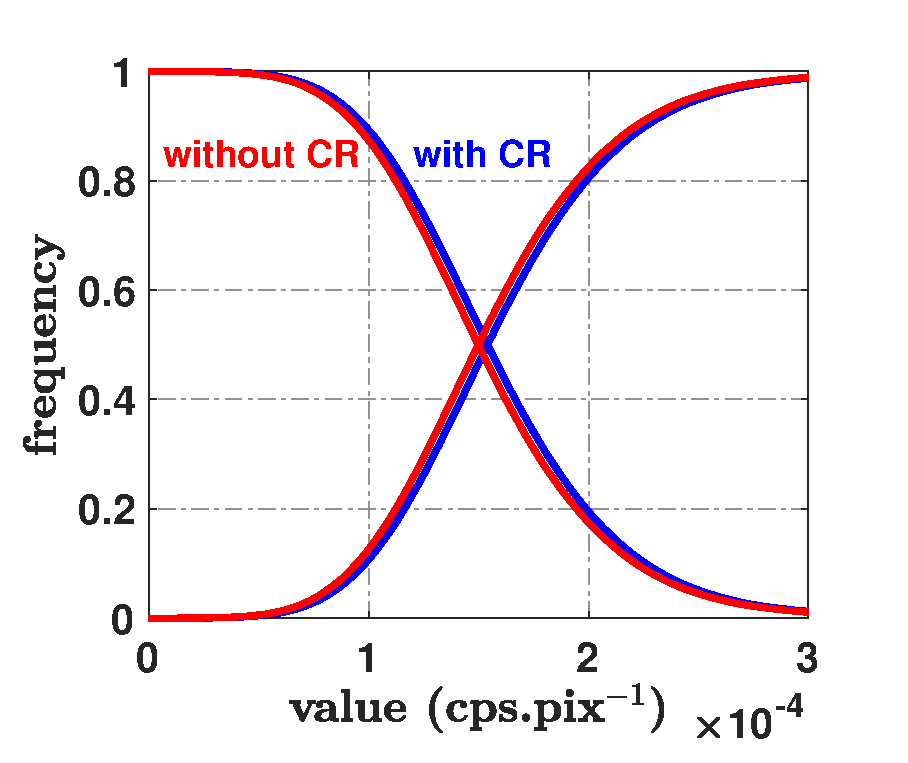
\includegraphics[width=0.4\linewidth]{fig6_CR/fig6B_CRCDF.eps}\label{fig:CR:B}} \qquad
\subfloat[C]{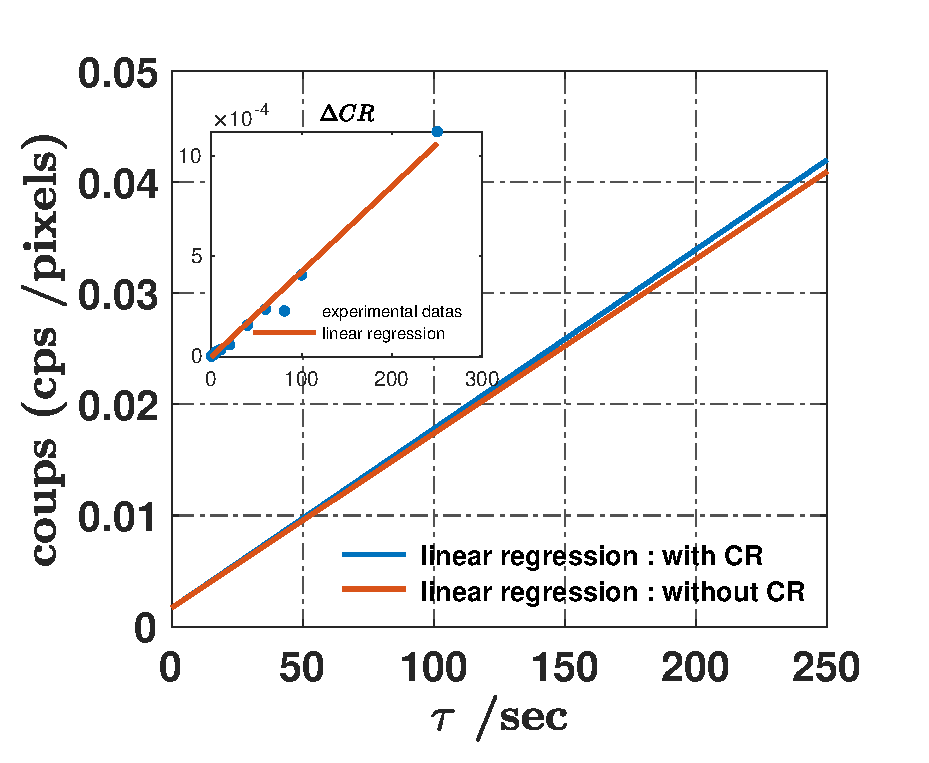
\includegraphics[width=0.4\linewidth]{fig6_CR/fig6C_CRfit.eps}\label{fig:CR:C}}


\caption{{\bf Cosmic Rays Frequency}. Aspect of a CR in a frame \subref{fig:CR:A}. The cumulative distributive function (CDF) and its complement of the frequency of counts \subref{fig:CR:B}, and the linear regression of the number of counts as a function of time is shown before and after removal of cosmic rays (CR) \subref{C}.  The experimental difference of the number of counts as a function of time before and after the removal of CR and its linear regression is on the insert of the figure \subref{fig:CR:C}.  }
\label{fig:CR}
\end{center}
\end{figure}

%%%%%%%%%%	
		%!TEX root = ../ArticleCalib_main.tex


%%%%%%%%%%%%% FIGURE 7 et 8 BBR theorique

\begin{figure}[htbp]
\begin{center}
\captionsetup[subfigure]{position=top, labelfont=bf, textfont=normalfont, singlelinecheck=off, justification=raggedright }

\subfloat[]{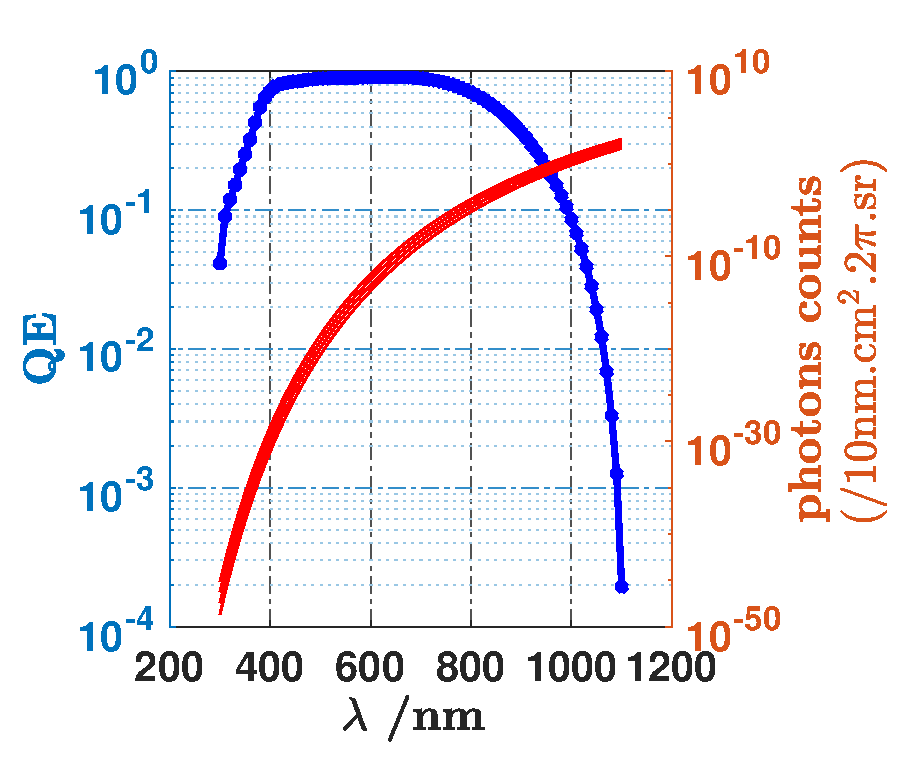
\includegraphics[width=0.4\linewidth]{fig7_8_BBRtheo/fig7A_nuvucamBBR15202530semilogy_QEdoubleax.eps}\label{fig:BBRtheo1:A}} \qquad
\subfloat[]{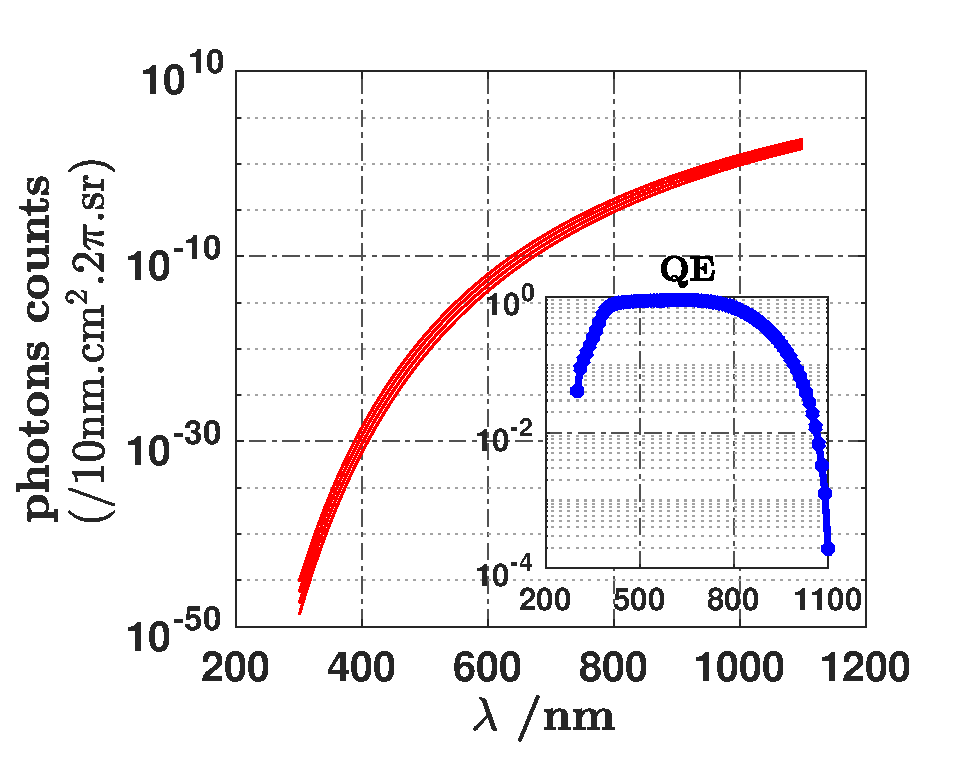
\includegraphics[width=0.4\linewidth]{fig7_8_BBRtheo/fig7A_nuvucamBBR15202530semilogy_QEinsert.eps}\label{fig:BBRtheo1:B}} \\

\subfloat[]{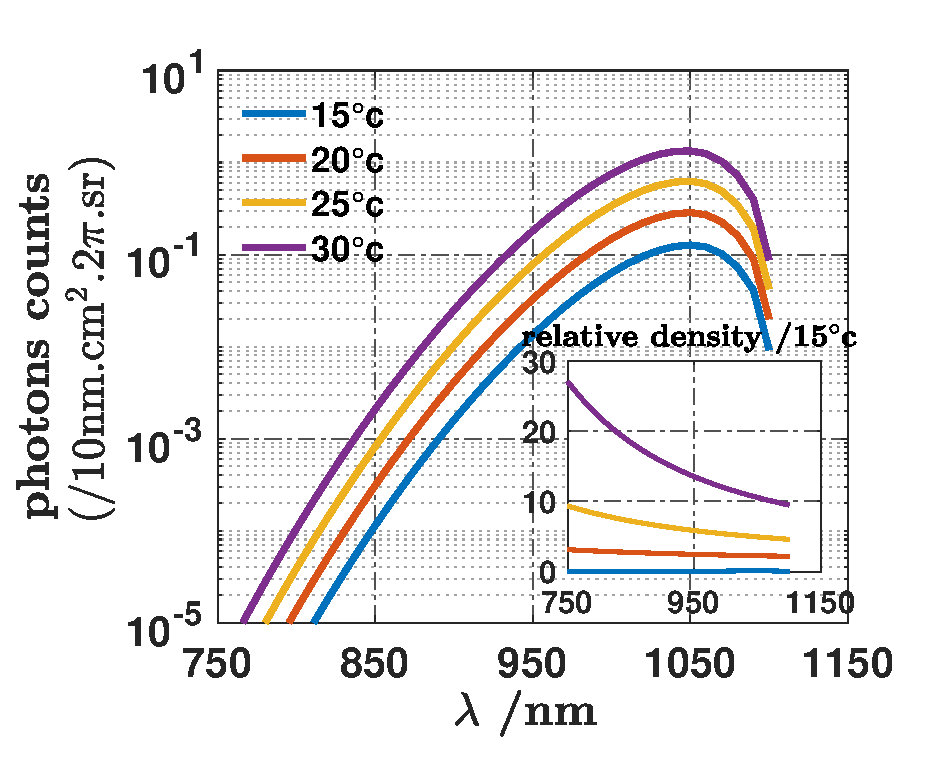
\includegraphics[width=0.4\linewidth]{fig7_8_BBRtheo/fig7B_nuvucamBBR_Tau600sPlanckBGsat_inclreldens15.eps}\label{fig:BBRtheo1:C}} \\

\subfloat[]{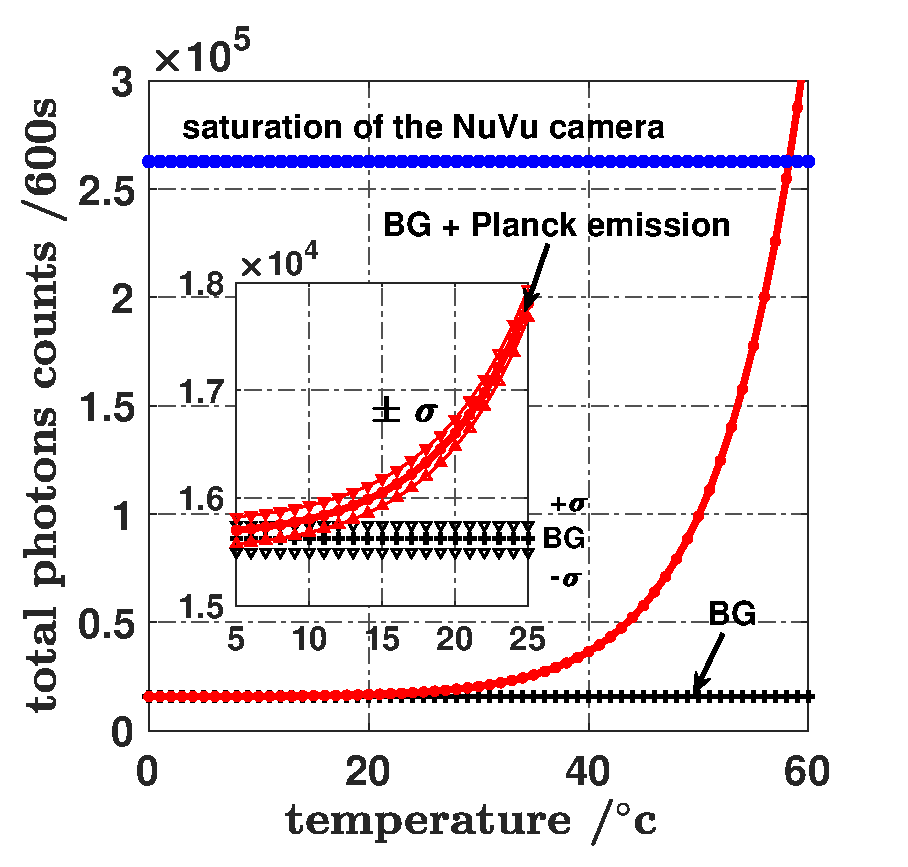
\includegraphics[width=0.5\linewidth]{fig7_8_BBRtheo/fig7C_nuvucamBBR_Tau600sPlanckBGsat_incl.eps}\label{fig:BBRtheo1:D}}

\caption{{\bf Black Body radiation spectra and spectral density of thermal radiation}.  The BBR is presented for increasing temperatures of 15, 20, 25 and 30 celsius degrees integrated over 10nm of wavelength during 1 second for 1 cm$^2$ surface over $2\pi$ sr. The inserted figure shows a zoom over $\lambda = [0.7 - 1.1]$ nm, representing the spectral density relative to 15$^o$c (\subref{fig:BBRtheo1:C}.)
{\bf Quantum Efficiency of the Nuvu Camera and spectral density of thermal radiation}.  Y axe is in logarithmic scale to show the dramatic decrease of the detectability when going toward shorter wavelength, the quantum efficiency of the NüVü camera is represented along with the spectral density of the thermal radiation.  (\subref{fig:BBRtheo1:A} and \subref{fig:BBRtheo1:B}.)
{\bf Model : NuVu Camera counts (N1) as a function of the temperature  }.  The N1 is given by summing the BackGround (BG) noise of the NuVu camera and the detected flux of the BBR. This detected flux is found by integrating the BBR over the QE as a function of $\lambda$ for a $\tau = 600s$. The pixels saturation level is shown ($N1 = \sum_{ij} pixels$). The inclusion shows the temperatures for which the detected Planck flux emission begins to be significantly detectable  (\subref{fig:BBRtheo1:D}.)}
\label{fig:BBRtheo1}
\end{center}
\end{figure}


\begin{figure}[htbp]
\begin{center}
\captionsetup[subfigure]{position=top, labelfont=bf, textfont=normalfont, singlelinecheck=off, justification=raggedright }

\subfloat[]{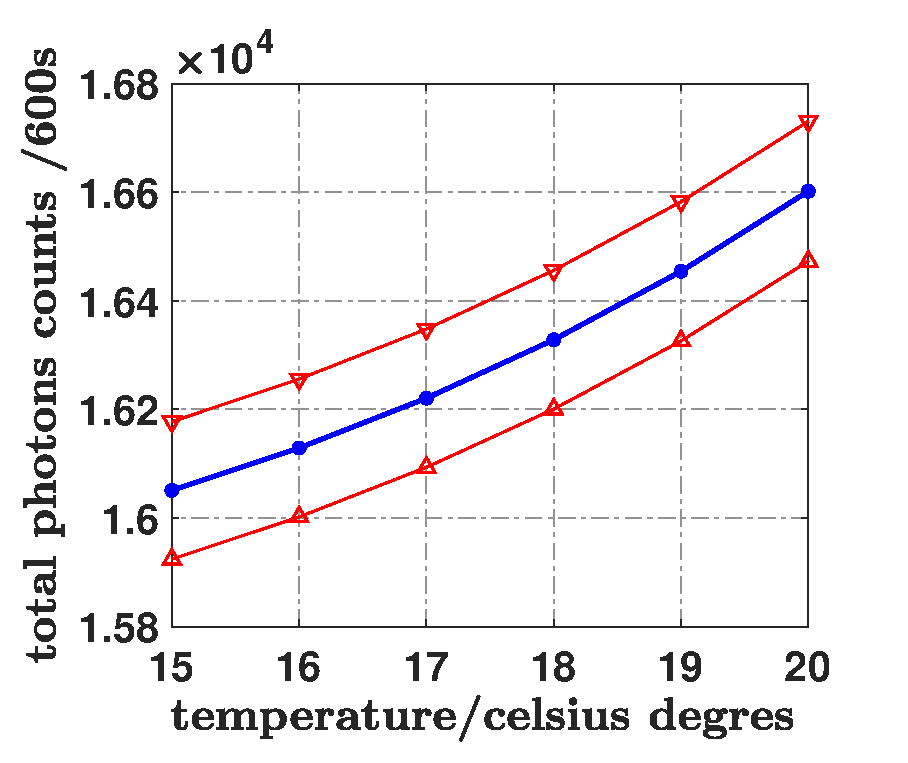
\includegraphics[width=0.4\linewidth]{fig7_8_BBRtheo/fig8A_nuvucamBBR_Tau600sPlanckTemp1520.eps}} \qquad
\subfloat[]{\includegraphics[width=0.4\linewidth]{fig7_8_BBRtheo/fig8B_nuvucamBBR_Tau600sPlanckTemp2025.eps}}\\

\subfloat[]{\includegraphics[width=0.4\linewidth]{fig7_8_BBRtheo/fig8C_nuvucamBBR_Tau600sPlanckTemp2530.eps}}\qquad
\subfloat[]{\includegraphics[width=0.4\linewidth]{fig7_8_BBRtheo/fig8D_nuvucamBBR_Tau600sPlanckTemp3035.eps}}\\

\subfloat[]{\includegraphics[width=0.4\linewidth]{fig7_8_BBRtheo/fig8E_nuvucamBBR_Tau600sPlanckTemp3540.eps}}\qquad

\caption{{\bf NuVu Camera counts (N1) as a function of the temperature : zoom}. Here is shown how the Noise Equivalent Temperature Difference (NETD) decrease dramatically with the increasing of the temperature. Arrows are showing the standard deviation of the measure according to the model. (A), (B), (C), (D), (E)  from [15 to 20], [20 to 25], [25 to 30], [30 to 35], [35 to 40] celsius degrees respectively. }
\label{fig:BBRtheo2}
\end{center}
\end{figure}



		%!TEX root = ../ArticleCalib_main.tex


%%%%%%%%%%%%% FIGURE 9 BBR theorique vs exp

\begin{figure}[htbp]
\begin{center}
\captionsetup[subfigure]{position=top, labelfont=bf, textfont=normalfont, singlelinecheck=off, justification=raggedright }

\subfloat[]{\includegraphics[width=0.4\linewidth]{fig9_BBRtheoExp/fig9A_BBR_plotsSumIJwithRCwithOLTau100s_BBRthoeFA.eps}\label{fig:BBRtheoexp:A}} \qquad
\subfloat[]{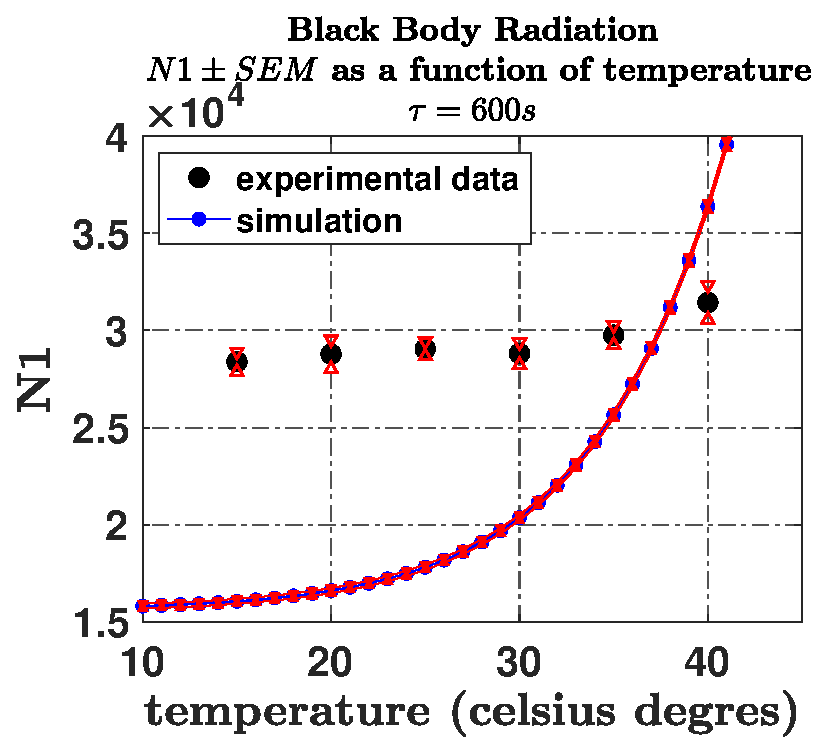
\includegraphics[width=0.4\linewidth]{fig9_BBRtheoExp/fig9B_BBR_plotsSumIJwithRCwithOLTau600s_BBRthoeFA.eps}\label{fig:BBRtheoexp:B}} \\

\subfloat[]{\includegraphics[width=0.4\linewidth]{fig9_BBRtheoExp/fig9C_BBR_plotsSumIJwithRCwithOLTau1000s_BBRthoeFA.eps}\label{fig:BBRtheoexp:C}} \\

\caption{{\bf Black Body radiation detection}.  The BBR is directly measured for increasing temperatures with different times of exposures (100 s (\subref{fig:BBRtheoexp:A}), 600 s (\subref{fig:BBRtheoexp:B}), 1000 s (\subref{fig:BBRtheoexp:A})), and compared to the simulation (\ref{fig:BBRtheo1}.)}
\label{fig:BBRtheoexp}
\end{center}
\end{figure}

		
%%%%%% EXPERIMENTAL RESULTS
	%\input{sections/articleCalib_section01_MM_laserCalib.tex}

	%%!TEX root = ../ArticleCalib_main.tex

%%%%%% CALIB LASER  article calib
\section{Experimental calibration}

		%!TEX root = ../ArticleCalib_main.tex


%%%%%%%%%%%%% FIGURE 14  DOUBLEMENT STOCH


%%%%%%%%%%%%% TAU 1s

\begin{figure}[htbp]
\begin{center}
\captionsetup[subfigure]{position=top, labelfont=bf, textfont=normalfont, singlelinecheck=off, justification=raggedright }

\subfloat[]{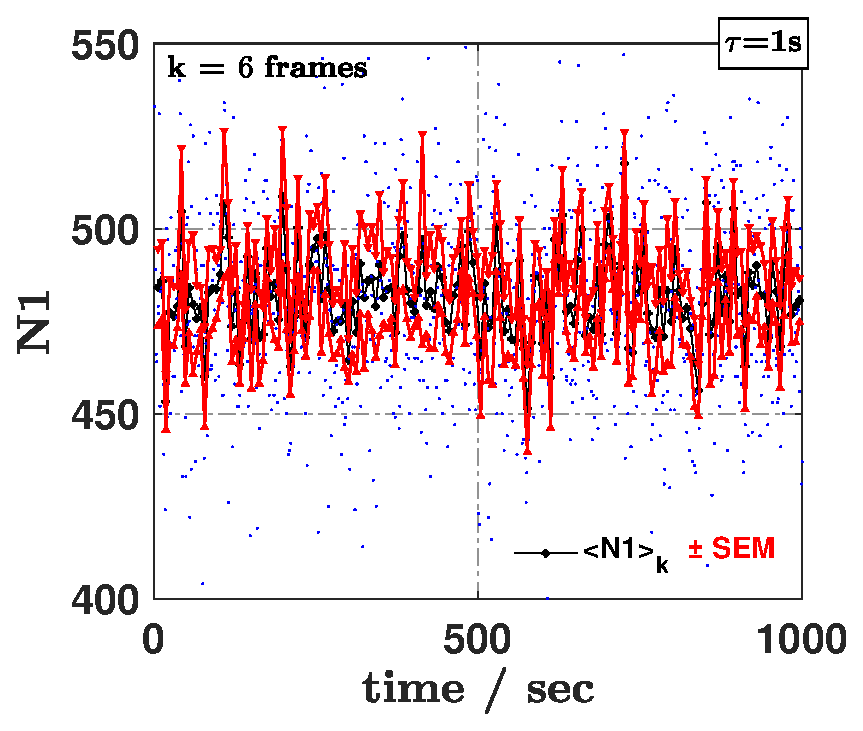
\includegraphics[width=0.4\linewidth]
	{fig14_doublementStoch/anlz191226_MeanSEM_BP_onk_doubleStoch_Tau1snoCRwithoutOutliers_1.eps}
	\label{fig:DoubleStoch:1s:A}} \qquad
\subfloat[]{\includegraphics[width=0.4\linewidth]
	{fig14_doublementStoch/anlz191226_MeanSEM_BP_onk_doubleStoch_Tau1snoCRwithoutOutliers_2.eps}
	\label{fig:DoubleStoch:1s:B}} \\

\subfloat[]{\includegraphics[width=0.4\linewidth]
	{fig14_doublementStoch/anlz191226_MeanSEM_BP_onk_doubleStoch_Tau1snoCRwithoutOutliers_3.eps}
	\label{fig:DoubleStoch:1s:C}} \qquad
\subfloat[]{\includegraphics[width=0.4\linewidth]
	{fig14_doublementStoch/anlz191226_MeanSEM_BP_onk_doubleStoch_Tau1snoCRwithoutOutliers_4.eps}
	\label{fig:DoubleStoch:1s:D}} \\

\subfloat[]{\includegraphics[width=0.4\linewidth]
	{fig14_doublementStoch/anlz191226_MeanSEM_BP_onk_doubleStoch_Tau1snoCRwithoutOutliers_5.eps}
	\label{fig:DoubleStoch:1s:E}} \qquad
\subfloat[]{\includegraphics[width=0.4\linewidth]
	{fig14_doublementStoch/anlz191226_MeanSEM_BP_onk_doubleStoch_Tau1snoCRwithoutOutliers_6.eps}
	\label{fig:DoubleStoch:1s:F}} \\






\caption{
{\bf Stochastic Filter ($\tau = $ 1s) }.  
During background camera measurement, moving average of the total counts on the sensor ($<N1>_k$) for  k data points (N1, blue dots) and its standard deviation of the mean (SEM) during $\tau=$1second. 
Increasing k shows that significative fluctuations are detectable during time while increasing the period until 200 seconds for a $\tau = $ 1s \subref{fig:DoubleStoch:1s:F}.
}
\label{fig:DoubleStoch:1s}
\end{center}
\end{figure}





%%%%%%%%%%%%%%%%%%%%%%%%% TAU 100sec
\begin{figure}[htbp]
\begin{center}
\captionsetup[subfigure]{position=top, labelfont=bf, textfont=normalfont, singlelinecheck=off, justification=raggedright }


\subfloat[]{\includegraphics[width=0.4\linewidth]
	{fig14_doublementStoch/anlz191226_MeanSEM_BP_onk_doubleStoch_Tau100snoCRwithoutOutliers_1.eps}
	\label{fig:DoubleStoch:100s:A}} \qquad
\subfloat[]{\includegraphics[width=0.4\linewidth]
	{fig14_doublementStoch/anlz191226_MeanSEM_BP_onk_doubleStoch_Tau100snoCRwithoutOutliers_2.eps}
	\label{fig:DoubleStoch:100s:B}} \\

\subfloat[]{\includegraphics[width=0.4\linewidth]
	{fig14_doublementStoch/anlz191226_MeanSEM_BP_onk_doubleStoch_Tau100snoCRwithoutOutliers_3.eps}
	\label{fig:DoubleStoch:100s:C}} \qquad
\subfloat[]{\includegraphics[width=0.4\linewidth]
	{fig14_doublementStoch/anlz191226_MeanSEM_BP_onk_doubleStoch_Tau100snoCRwithoutOutliers_4.eps}
	\label{fig:DoubleStoch:100s:D}} \\

\subfloat[]{\includegraphics[width=0.4\linewidth]
	{fig14_doublementStoch/anlz191226_MeanSEM_BP_onk_doubleStoch_Tau100snoCRwithoutOutliers_5.eps}
	\label{fig:DoubleStoch:100s:E}} \qquad
\subfloat[]{\includegraphics[width=0.4\linewidth]
	{fig14_doublementStoch/anlz191226_MeanSEM_BP_onk_doubleStoch_Tau100snoCRwithoutOutliers_6.eps}
	\label{fig:DoubleStoch:100s:F}} \\


\caption{
{\bf Stochastic Filter ($\tau = $ 100s) }.  
During background camera measurement, moving average of the total counts on the sensor ($<N1>_k$) for  k data points (N1, blue dots) and its standard deviation of the mean (SEM) during $\tau=$100second. 
Increasing k shows that significative fluctuations are detectable during time while increasing the period until 8000  seconds for a $\tau = $ 100s \subref{fig:DoubleStoch:100s:F}.
}
\label{fig:DoubleStoch:100s}
\end{center}
\end{figure}






		%!TEX root = ../ArticleCalib_main.tex


%%%%%%%%%%%%% FIGURE 10  Calibration experimentale laser & Corrélations

\begin{figure}[htbp]
\begin{center}
\captionsetup[subfigure]{position=top, labelfont=bf, textfont=normalfont, singlelinecheck=off, justification=raggedright }

\subfloat[]{\includegraphics[width=0.4\linewidth]{fig10_CalibExp_Correlation/fig10A_BGBG_CorrelationsProches_fluctuations.pdf}\label{fig:CalibCorrel:A}} \qquad
\subfloat[]{\includegraphics[width=0.4\linewidth]{fig10_CalibExp_Correlation/fig10B_CalibLaser.pdf}\label{fig:CalibCorrel:B}} 

\subfloat[]{\includegraphics[width=0.7\linewidth]{fig10_CalibExp_Correlation/fig10C_CalibLaser.pdf}\label{fig:CalibCorrel:C}} \\



\caption{
{\bf Experimental calibration and noise subtraction to free measurement from low frequencies noise variations}. 
\subref{fig:CalibCorrel:A} : Raw data taken in the most possible darkness on the entire surface sensor, (ie shutter closed), (N1$_{BG}$) show a slow relaxation process. 
When subtracting neighbouring data points (N1$_{\Delta BG}$),  the observed variance is lower than the expected variance for non correlated measurements, and only high frequency fluctuation from the camera sensor noise remains (variation between two neighbouring points).
The distribution of both set of data point is respectively shown by the histograms.
\subref{fig:CalibCorrel:B} : Calibrated flux detection with the NuVu camera and comparaison of the experimental results and the model describing the behavior of the NuVu camera.
The datas are the average of the difference between the average photons counts inside the area illuminated by the laser  beam (40 mm²  diameter disk) during the  time of exposure of optimal density  (160sec), and  the environmental noise (determined with the shutter open while the LASER is off). 
All statistics are made on the difference between the signal (camera shutter open) and the camera noise (camera shutter closed : BG).
The limit of detection (black dotted line) represents the noise floor, and corresponds to $5.8 counts /\mathrm{cm}^{-2}s$.
\subref{fig:CalibCorrel:C}  : Experimental setup to produce a beam of calibrated low light fluxes. The final optical elements are placed in a thorlab SM1 tube and fixed on the camera via c-mount. 
We only select the central zone of the infinite attenuated beam to have a better average flux uniformity throughout the beam section.
}
\label{fig:CalibCorrel}
\end{center}
\end{figure}

		


\end{document}



